%% LyX 2.1.2 created this file.  For more info, see http://www.lyx.org/.
%% Do not edit unless you really know what you are doing.
\documentclass[a4paper,UTF8,winfonts]{ctexbook}
\usepackage[T1]{fontenc}
\setcounter{secnumdepth}{3}
\setcounter{tocdepth}{3}
\usepackage{color}
\definecolor{shadecolor}{rgb}{0.667969, 0.667969, 0.5}
\usepackage{fancybox}
\usepackage{calc}
\usepackage{framed}
\usepackage{amsmath}
\usepackage{graphicx}
\usepackage[unicode=true,
 bookmarks=true,bookmarksnumbered=true,bookmarksopen=true,bookmarksopenlevel=0,
 breaklinks=false,pdfborder={0 0 0},backref=false,colorlinks=false]
 {hyperref}

\makeatletter

%%%%%%%%%%%%%%%%%%%%%%%%%%%%%% LyX specific LaTeX commands.
\pdfpageheight\paperheight
\pdfpagewidth\paperwidth

%% Because html converters don't know tabularnewline
\providecommand{\tabularnewline}{\\}
%% A simple dot to overcome graphicx limitations
\newcommand{\lyxdot}{.}


\@ifundefined{date}{}{\date{}}
%%%%%%%%%%%%%%%%%%%%%%%%%%%%%% User specified LaTeX commands.
% 如果没有这一句命令,XeTeX会出错,原因参见
% http://bbs.ctex.org/viewthread.php?tid=60547
\DeclareRobustCommand\nobreakspace{\leavevmode\nobreak\ }

\usepackage{algpseudocode}

\makeatother

\usepackage{listings}
\renewcommand{\lstlistingname}{列表}

\begin{document}

\title{算法笔记}


\author{http://www.csie.ntnu.edu.tw/}

\maketitle

\section*{关于算法笔记}


\subsection*{本站介绍}

本站数据是基于分享的精神,一字一句累积起来的。个人希望藉由此站,分享所学所得,支持计算器科学发展。

本站尚处创建阶段,内容不够详尽周全。各位读者若发现错误,欢迎利用留言板告知,俾能改正,十分感谢。

大家可以自行撷取本站的图文作各种用途。想想天地,摸摸良心,不要拿去为非作歹、谋取私利就可以了。 


\subsection*{工作项目}


\subsubsection*{过去工作项目}
\begin{enumerate}
\item 提供算法教学数据。将常见的算法分门别类、编纂目录,归纳一套完整的理论系统。
\item 推广算法解题。收集大量的算法练习题目,穿插于本站的教学数据当中,例如 \href{http://uva.onlinejudge.org/}{UVa Online Judge},藉此提升学生的程序设计能力。
\item 宣传算法竞赛。例如 \href{http://icpc.baylor.edu/}{ACM-ICPC}、\href{http://code.google.com/codejam/}{Google Code Jam}、\href{http://community.topcoder.com/tco13/}{TopCoder Open}
等等,增加学生的国际交流经验。
\item 出版算法设计的书籍:\href{http://www.drmaster.com.tw/Bookinfo.asp?BookID=PG21318}{培养与锻炼……基础入门},推广算法设计的观念。书中内容现在已经汇整至网站上了。
\item 引进国外学校有教,但是国内学校没有教的算法。例如\href{http://courses.csail.mit.edu/6.851/}{高等数据结构}、\href{http://courses.csail.mit.edu/6.854/}{高等算法}、\href{http://www.ics.uci.edu/~eppstein/163/}{图论算法}、\href{http://www-math.mit.edu/~goemans/teaching.html}{组合优化}、\href{http://cs.smith.edu/~orourke/}{计算几何}、\href{http://www.inf.kcl.ac.uk/staff/mac/}{字符串学}等等,将重要的算法知识介绍给国内学子。
\end{enumerate}

\subsubsection*{当前工作项目}
\begin{enumerate}
\item 介绍\href{http://zh.wikipedia.org/wiki/\%E8\%AE\%A1\%E7\%AE\%97\%E6\%9C\%BA\%E7\%A7\%91\%E5\%AD\%A6}{计算机科学}的应用。收集相关影片,让大众了解计算机科学有什么功用、计算机科学如何改善生活环境。
\item 整理媒体算法。例如\href{http://en.wikipedia.org/wiki/Text_processing}{文字处理}、\href{http://en.wikipedia.org/wiki/Audio_signal_processing}{声音处理}、\href{http://en.wikipedia.org/wiki/Image_processing}{图像处理}、\href{http://en.wikipedia.org/wiki/Computer_graphics}{计算机绘图}、\href{http://en.wikipedia.org/wiki/Computer_vision}{计算机视觉}以及各种进阶领域,拓展信息人的视野。
\end{enumerate}

\subsubsection*{预计工作项目}
\begin{enumerate}
\item 将网站译为其它语言,让更多人可以获取网站资源。
\item 汇整各种计算机科学领域所对应的软件公司,藉此促进人才媒合,也藉此让在学学生了解产业现况、培养志向。
\item 探讨如何运用计算机科学改善社会问题、增进民众福祉。
\end{enumerate}

\subsection*{资助算法笔记}

站长家庭经济状况不佳,日子过得清澹。如果每个月有稳定薪资,就不必烦恼经济问题──然而没有人提供编写算法笔记的工作,站长必须常常分神去从事其它工作。

理想的方式,是由政府或富人,每月固定资助新台币 35000 元做为薪资,让站长可以全心投入算法笔记。愿意资助的朋友,请来信 algorithm.notes@gmail.com
。 

站长的眼睛已经渐渐好转,现在可以长时间使用计算机,不过写程序的话还是太吃力了。因此麻烦大家别再推荐程序开发的工作了! 

\tableofcontents{}


\part{Algorithm}


\chapter{Algorithm}


\section{Algorithm}


\subsection{算法是什么}

算法是资讯工程系非常重要的基础科目。简单来说,算法就是用计算机算数学的学问(古代人用算盘算、现代人用计算机算),可以说是数学科目。

想要解决现实生活当中的各种问题,计算机科学家就把现实问题对应到数学问题,然后设计公式、把公式写成程序,让计算机执行程序计算答案──这些公式就叫做算法了。

尽管这里用了「公式」这个字眼来形容算法,然而并不是各位印象中的数学公式。由于计算机能够执行繁复的计算,所以公式可以设计成好几十行、好几百行,甚至用到很多数学理论。

因此呢,就算学习过算法的人,也不见得懂得设计算法;因为数学、程序的东西实在太复杂了。想把现实问题对应到数学问题,那就更复杂了。


\subsection{计算机只会算数字}

回过头来,计算机又是什么?计算机是个很潮的中文翻译,不过实际上计算机的原意是「计算机」。计算机的英文叫做 computer ,而计算的英文就叫做
compute 。 计算机是一台计算机,只会计算、判断、储存数字。又快又准。 程序是一连串计算、判断、储存数字的步骤。 计算机只会处理数字(二进制数)。计算机里的每一个文字、每一种颜色、每一种声音,其实都有相对应的数字。
打个比方,我们规定:用 1 代表「一」,用 2 代表「乙」,用 3 代表「人」,……。一个数字对应一个中文字。计算机里面的所有中文字,都依循人为规定,变作了数字。
再打个比方,「人」这个字,呈现计算机屏幕上是个「人」样。计算机屏幕的画面,是由许多小光点组成的;计算机屏幕上的「人」也是由许多小光点组成的。我们以「人」的左下角为坐标原点,横向为
X 轴,直向为 Y 轴,那么「人」其实是 (0,1) 、 (1,2) 、 (2,3) 、 ... 这些坐标画上黑点后所形成的。「人」这个字的的形状,在计算机中变作了一连串的数字。

同样的道理,呈现在计算机屏幕画面上的文字、颜色、图片、影像、声音,全部都可以化作数字。一切事物在计算机里面都是数字。 计算机并没有想象中的那么神奇。不过计算机最厉害的地方并不是计算机本身,而是在于计算机可以接上各式各样的设备。接上摄影机与屏幕,就可以把色彩变成数字、把数字变成色彩;接上麦克风与耳机,就可以把声音变成数字、把数字变成声音。

计算机一旦接上了设备,就额外有用处。接上话机和基地台,就可以互通有无;接上数字相机和打印机,就可以制造回忆;接上重量仪和筛子,计算机也会拣土豆;接上车厢、接上警示灯、再杂七杂八接上一堆东西,就变成了大众运输系统。

若要用计算机解决现实问题,通常要考虑两个方面:一、计算机应该接上那些设备?如何用计算机控制这些设备?二、现实问题如何对应到数学问题?如何设计算法? 


\subsection{程序用来比对数字、改变数字、储存数字}

举个例子,我们希望把屏幕上的「人」变成斜体字。过程大略是这样──首先呢,把「人」的形状 (0,1) 、 (1,2) 、 (2,3)
、 ... 这些数字拿出来;然后呢,位置越高的坐标,就往右移动多一点,如此一来就成为斜体字了。想让坐标往右移动,就是让计算机做数字加法计算,然后把相加结果储存起来。

再举个例子,用鼠标点选一个文件夹,文件夹的颜色会反白。过程大略是这样──首先呢,计算机侦测到鼠标点击的坐标之后,把坐标转换成数字;然后呢,再把屏幕画面的数据拿出来,看看屏幕上每个东西的坐标,是哪一个与鼠标的坐标相符合;噢,原来是一个文件夹的图标,把文件夹的显示颜色给反白过来。

再举个例子,计算机据说会拣选土豆。过程大略是这样──把每一颗土豆拿出来,利用特殊的仪器,把形状、重量、色泽、气味统统转换成数字,储存在计算机里面;然后呢,用计算机比较这些数字,找出优良的土豆,如此一来就有绵绵松松的土豆了!
编写程序,计算数字,这就是程序设计师的工作。 


\subsection{数学和程序这么复杂,为什么要用计算机解决现实问题?}

计算机的计算速度可说是非常的快,一秒钟可以进行好几千万次。就算文字多么的多,图片多么的大,计算机处理起来,也是轻松写意,顺畅无比。

打开计算机里的任何一份文件,用鼠标卷动一下文件画面,眼睛都还没眨一下,正确画面马上就呈现在屏幕上了。事实上在卷动画面的时候,计算机已经经过几千万次的计算,仅使用了极短的时间,就把屏幕上应该呈现的数据全部计算好了。

人类会想要用计算机解决问题,正是仰赖计算机的计算速度、正确性,以及计算机会自动按照程序计算的特性。程序设计师只要花心思写出一支好程序,接下来的工作就可以让计算机代劳了。计算机做的比人类更快更好,计算机做得到人类做不到的事情;尽管数学和程序很复杂,还是有很多人选择使用计算机解决问题。 


\section{Algorithm}


\subsection{算法是什么?}

\href{http://zh.wikipedia.org/wiki/\%E6\%BC\%94\%E7\%AE\%97\%E6\%B3\%95}{算法}由三个部分组成:输入、计算步骤、输出。介绍这件事情的时候,有人连结到\href{http://zh.wikipedia.org/wiki/\%E5\%87\%BD\%E6\%95\%B8}{函数}的概念,也有人连结到\href{http://zh.wikipedia.org/wiki/\%E9\%BB\%91\%E7\%AE\%B1}{黑箱白箱}的概念。

输出、输入是一堆数字。实务上是将这些数据放在数据结构,例如 array 、 linked list 。

输入数据的来源,通常是硬盘里面储存的档案,或者是藉由硬件装置撷取到的数据,例如数字相机、麦克风等等。输出数据的去处,通常是硬盘里面储存的档案,或者是藉由硬件装置转换之后以其它型态呈现,例如数字电视、数字音响等等。 

\noindent %
\shadowbox{\begin{minipage}[t]{1\columnwidth}%
加法的算法

a --- {[} {]} ---> c 

b ---

例如

5 --- {[} {]} ---> 8 

3 --- %
\end{minipage}}

计算步骤有两种类型,一类是运算,例如数学运算加减乘除、逻辑运算且或非、比较运算大于等于小于。另一类是读写,例如读取某处的数字、储存数字至某处,就跟计算机的
MR 、 M+ 按键的意义相似。

古人定义算法,规定计算步骤的数量是必须是有限步,不是无限步。用程序语言的术语来说就是:算法不能有无穷循环。

古人当初规定有限步,是为了方便统计总步数。但是实务上,很多计算机程序是开启之后就保持执行状态,直到当机、重开机,例如网络传输的算法。因此实务上可以是无限步。 


\subsection{如何记载一个算法?}

有人用\href{http://zh.wikipedia.org/wiki/\%E4\%BC\%AA\%E4\%BB\%A3\%E7\%A0\%81}{伪码}来记载一个算法。如要设计\href{http://zh.wikipedia.org/wiki/\%E8\%AE\%A1\%E7\%AE\%97\%E6\%9C\%BA\%E7\%A8\%8B\%E5\%BA\%8F}{计算机程序},伪码是比较恰当的。

\noindent \begin{algorithmic}[1]
\Procedure{Greatest\_{}Common\_{}Divisor}{$a,b$}
    \While{$a\neq b$}
        \If{$a > b$}
            \State $a\gets a-b$
        \Else
            \State $b\gets b-a$
        \EndIf
    \EndWhile
\State \textbf{return} $a$
\EndProcedure
\end{algorithmic}

有人用流程图来记载一个算法。如要设计电子电路,流程图是比较恰当的。

\begin{center}
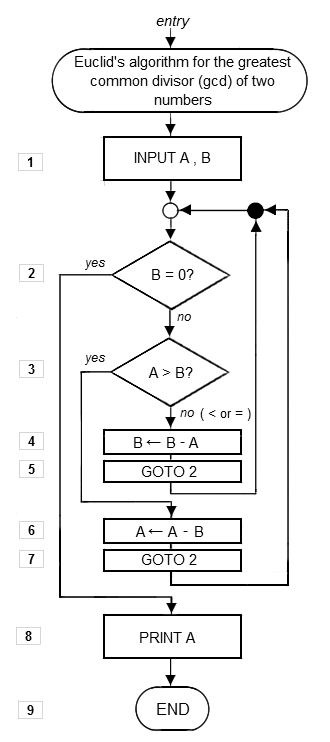
\includegraphics[scale=0.6]{images/Euclid_flowchart_1}
\par\end{center}

大多数时候,我们无法光从伪码和流程图彻底理解算法,就如同我们无法光从数学公式彻底理解数学概念。想要理解算法,通常还是得藉由文字、图片的辅助说明。


\subsection{如何实作一个算法?}

实作的意思是:实际去操作、实际去运行。对于资工系学生来说,自然就是把算法撰写成计算机程序,例如 C 或者 C++ 程序语言,然后在个人计算机上面执行程序。

\noindent 
\begin{lstlisting}[language=C,numbers=left,basicstyle={\ttfamily}]
int gcd(int a, int b) {
    while (a != b)
        if (a > b)
            a -= b;
        else
            b -= a;
    return a;
}
\end{lstlisting}


对于电机系学生来说,自然就是把算法设计成\href{http://zh.wikipedia.org/wiki/\%E9\%9B\%BB\%E5\%AD\%90\%E9\%9B\%BB\%E8\%B7\%AF}{电子电路},在\href{http://zh.wikipedia.org/wiki/\%E9\%9D\%A2\%E5\%8C\%85\%E6\%9D\%BF}{面包板}、\href{http://zh.wikipedia.org/wiki/\%E5\%8D\%B0\%E5\%88\%B7\%E9\%9B\%BB\%E8\%B7\%AF\%E6\%9D\%BF}{印刷电路板}、
\href{http://zh.wikipedia.org/wiki/\%E5\%8F\%AF\%E7\%A8\%8B\%E5\%BC\%8F\%E9\%82\%8F\%E8\%BC\%AF\%E8\%A3\%9D\%E7\%BD\%AE}{PLD}
上面执行。

电子电路也有加法器、减法器、 AND 逻辑闸、 OR 逻辑闸等等,所以也可以用电子电路实作算法。例如电子表、随身听、悠游卡等等,都是直接将算法做死在芯片上面。在个人计算机、智能型手机还没流行之前,以往都是用电子电路实作算法。

\noindent 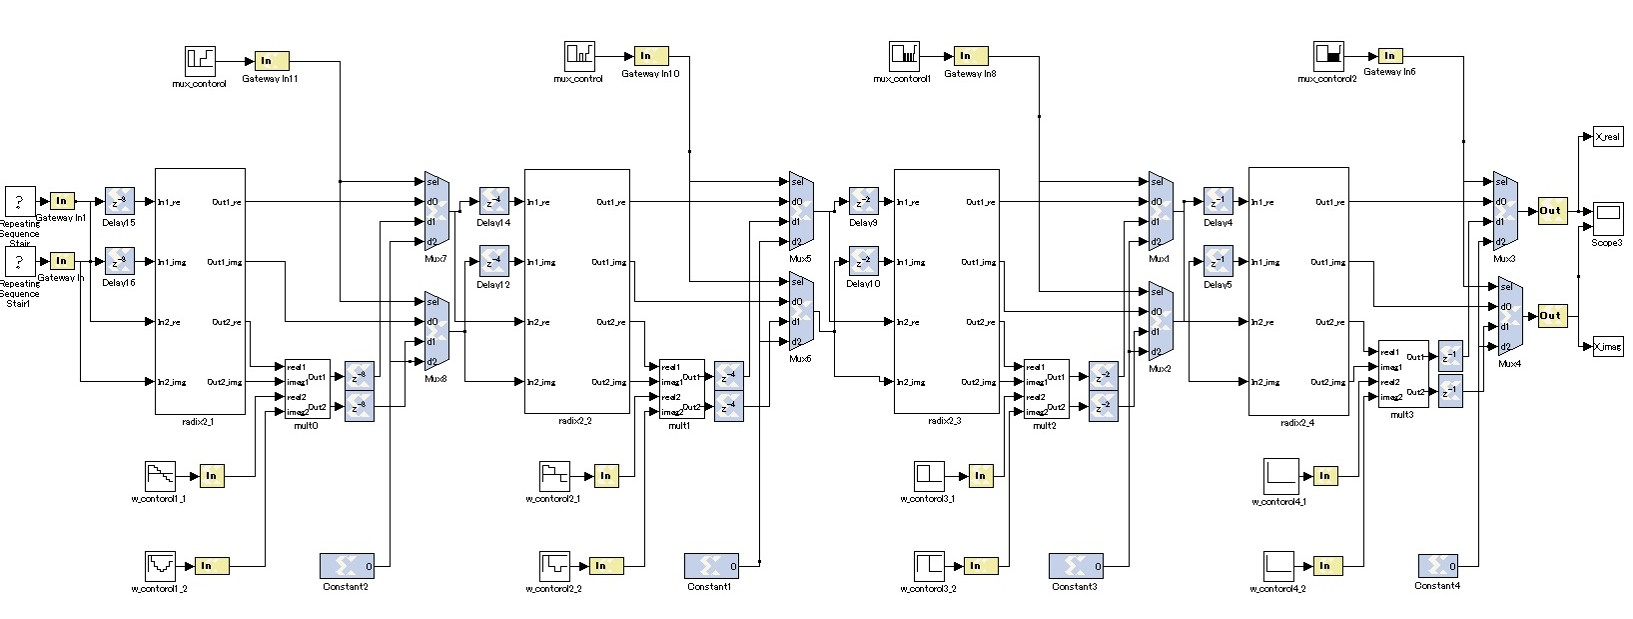
\includegraphics[scale=0.25]{images/fig34_large}

电子电路的执行速度是飞快的,计算机程序的执行速度慢了一点。制作电子电路的过程相当麻烦,需要精密的设备、复杂的制程、大量的人力和经费,而且制成之后就无法修改;但是写程序就简单轻松多了。相对地,在计算机上面很容易调整程序代码,又可以储存很多程序代码,最主要的是家家户户都有计算机。


\subsection{时间复杂度、空间复杂度}

要评断一个算法的好坏,最基本的指标是时间和空间。

最直觉的方式,就是测量程序的执行时间、程序的内存使用量。但是由于同一个算法在不同计算机上面的执行时间稍有差异,又由于每个人实作算法所采用的程序语言、程序设计技巧都不一样,所以执行时间、内存使用量不是一个稳定的评断标准。

数学家于是计算步骤数量。 \begin{algorithmic}[1]
\Procedure{BubbleSort}{$A$}
    \For{$i\gets 0, length(A)-1$}
        \For{$j\gets 0, length(A)-i-1$}
            \If{$A[j] < A[j+1]$}
                \State swap A[j] and A[j+1]
            \EndIf
        \EndFor
    \EndFor
\EndProcedure
\end{algorithmic}%
\begin{minipage}[t]{1\columnwidth}%
\begin{shaded}%
\begin{algorithmic}[1]
\Procedure{BubbleSort}{$A,n$}
    \For{$i\gets 0, n-1$}\Comment{$n$}
        \For{$j\gets 0, n-i-1$}\Comment{$\frac{n(n-1)}{2}$}
            \If{$A[j] < A[j+1]$}\Comment{$\frac{n(n-1)}{2}$}
                \State $temp\gets A[j]$\Comment{$\frac{n(n-1)}{2}$}
                \State $A[j]\gets A[j+1]$\Comment{$\frac{n(n-1)}{2}$}
                \State $A[j+1]\gets temp$\Comment{$\frac{n(n-1)}{2}$}
            \EndIf
        \EndFor
    \EndFor
\EndProcedure
\end{algorithmic}\end{shaded}%
\end{minipage}

$\begin{aligned}total & =n+\frac{5n(n-1)}{2}\\
 & =n+2.5n^{2}-2.5n\\
 & =2.5n^{2}-1.5n\\
 & =O(n^{2})
\end{aligned}
$

数学家把步骤数量写成代数式子。例如当数据有 $n=1000$ 笔,步骤数量一共是 $2.5\times1000^{2}-1.5\times1000=2498500$
步。

有了步骤数量之后,还可以进一步粗估执行时间。假设一个步骤需要 10 个 clock,而计算机中央处理器 CPU 的频率是 2GHz
:每秒钟执行 2000000 个 clock,那么程序执行时间大约 12.4925 秒。

但是这不是精准的步骤数量。由于实作的关系,系数很容易变动,所以系数的意义不大。因此数学家只取出代数式子的最高次方,并且规定 $n$
必须足够大(类似微积分的极限概念)。尽管这是非常不精准的估算方式,不过还是可以对常见的算法进行简易分类,粗略地比较快慢。

\noindent \begin{center}
\begin{minipage}[t]{1\columnwidth}%
\begin{center}
\begin{tabular}{|c|c|c|}
\hline 
 & time{*} & space\tabularnewline
\hline 
\hline 
bubble sort & $O(n^{2})$ & $O(n)$\tabularnewline
\hline 
insertion sort & $O(n^{2})$ & $O(n)$\tabularnewline
\hline 
merge sort & $O(n\log(n))$ & $O(n)$\tabularnewline
\hline 
quicksort & $O(n^{2})$ & $O(n)$\tabularnewline
\hline 
heapsort & $O(n\log(n))$ & $O(n)$\tabularnewline
\hline 
counting sort & $O(n+r)$ & $O(n+r)$\tabularnewline
\hline 
\end{tabular}
\par\end{center}

\begin{center}
{*}worst case
\par\end{center}%
\end{minipage}
\par\end{center}

空间的计算方式与时间类似,就不多提了。由于空间复杂度不会超过时间复杂度,而且空间复杂度通常不会呈指数成长,所以大家比较不在意空间复杂度。教科书上面通常比较强调时间复杂度。


\subsection{解决问题的成效}

算法的好坏除了时间和空间的用量以外,主要还是看算法解决问题的成效如何。

数学问题,通常可以明定解答好坏,例如数字越大越好。通常这种情况,有多种算法可以求得正解,那么这些算法的成效是一样好的。

真实世界的问题,通常难以界定绝对的好坏优劣,例如美丑、乐音噪音、喜怒哀乐、是非对错等等,此时算法的成效,就由人自行判断,利用两两比较、投票表决等等方式来决定成效。 


\section{Algorithm}


\subsection{学习程序语言}

学习程序语言,有两个层次:一、程序语言本身的语法;二、把想法转换成程序代码。

第一个层次即是「程序语言 Programming Language 」。终极目标是背熟规格书、灵活运用程序语言。可参考本站文件「\href{http://www.csie.ntnu.edu.tw/~u91029/C++.html}{ C/C++}」。

第二个层次即是「程序设计 Programming 」。终极目标是设计程序代码解决问题。可参考本站文件「\href{http://www.csie.ntnu.edu.tw/~u91029/Programming.html}{ Programming}
」。 


\subsection{学习算法}

学习算法,有两个层次:一、算法本身的运作过程;二、把想法转换成算法。

第一个层次即是「算法 Algorithm 」。终极目标是灵活运用各个算法。可参考本站首页的各大字段,例如图论、计算几何、字符串学等等。

第二个层次即是「算法设计 Algorithm Design 」。终极目标是设计数学计算解决问题。可参考本站首页的 Algorithm
Design 字段。 


\subsection{算法设计、算法分析}

算法又可以细分为两个不同的方向。

算法设计,是制造相对应的算法。算法设计目前已经有一些经典手法,例如 Dynamic Programming 、 Greedy 等等。读者可以参考《
\href{http://www.aw-bc.com/info/kleinberg/}{Algorithm Design} 》这本书。

算法分析,是针对特定算法,精确计量时间复杂度和空间复杂度。算法分析会用到很多数学知识。读者可以参考《 \href{http://aofa.cs.princeton.edu/home/}{An Introduction to the Analysis of Algorithms }》这本书。 


\section{Algorithm Class}


\subsection{Offline Algorithm / Online Algorithm}

「离线算法」是一口气输入所有数据之后,才能开始运行的算法。例如 Bubble Sort 。

「在线算法」是不需等待所有数据到达,就可以分时分段处理输入的算法。例如 Insertion Sort 。

有些「在线算法」甚至可以实时提供目前所有输入的正确输出。例如 Insertion Sort 。


\subsection{Static Algorithm / Dynamic Algorithm}

「静态算法」是无法随时修改、增加、减少原本的输入数据,无法随时查询输出的算法。例如 Dijkstra's Algorithm 。

「动态算法」是可以随时修改、增加、减少原本的输入数据,可以随时查询输出的算法。例如 Binary Search Tree 。 


\subsection{Exact Algorithm / Approximation Algorithm}

「精确算法」是计算结果绝对正确的算法。

「近似算法」是计算结果拥有误差的算法。

有许多问题无法快速计算正确答案。为了追求速度,就会设计「近似算法」。 


\section{Time Complexity }


\subsection{时间复杂度}

想要描述一个算法执行速度有多快,最直觉的方式是测量算法计算时间,另一种方式是统计算法步骤数目。由于执行时间深受机械规格与实作方式影响,难以放诸四海皆准,因此学术上倾向于统计算法步骤数目。一般都是统计加减乘除的次数。


\subsection{时间复杂度标记法}

时间复杂度的标记法,是几十年前的数学家发明的一种方式:大写的英文字母 $O$ 函数代表算法执行步骤数目上限,大写的希腊字母 $\varOmega$
函数代表下限,大写的希腊字母 $\varTheta$ 函数代表同时满足上限与下限(也就是不多不少刚刚好)。这些都是假设 $N$
无限大的情况,又由于 $N$ 无限大,所以我们只需比较函数的最高次方项,另外我们省略了最高次方项的系数。

$N$ 无限大。无限大对数学家来说是司空见惯,然而对程序设计师来说却是天方夜谭。什么时候程序设计师才会遇到无限大的测试数据呢?遇不到。真实世界中根本不可能把无限大的测试数据输入到程序之中。不管是什么坚忍不拔、屹立不摇的程序,总还是有那么一天,发生了停电、当机、人为更新设备,而把程序中止了,造成程序没时间吃进无限多的测试数据。真实世界也没有那么大的内存能够一口气读进无限多笔数据。
$N$ 无限大是不可能的,但是有可以模拟为 $N$ 无限大的情况。例如操作系统的程序,例如网络应用程序,持续执行个一年半载都不停,含辛茹苦不眠不休地处理数据。一有测试数据就赶快解决掉,当作好像没有发生过一样,乍看是无限多笔测试数据,实际上却是同一个步骤执行无限多次。这时候用时间复杂度的标记法,用来判断算法快慢,是一个不错的指标。然而还是要小心,当两个算法时间复杂度一样,两者的速度也可能相去甚远,因为最高次方项的系数根本就被忽略了。
一般在单机上跑没几秒钟就会结束的程序,只喂那少少的测试数据,要拿时间复杂度来评定算法快慢,那就有点扯了。 $N=5$ 的情况下,说不定
$O(N^{3})$ 的算法表现的比 $O(N^{2})$ 好。设计一个 $O(N)$ 的算法,在 $N=5$ 的情况下反而跑的比
$O(N^{2})$ 的算法还慢。两个同为 $O(N)$ 的算法可能不一样快,$N$ 大时甲快、 $N$ 小则乙快。 


\subsection{测试数据}

当测试数据很乱,那我们可以说平均的时间复杂度多少;当测试资料很整齐,那我们可以说最佳与最坏的时间复杂度为多少。例如 Quicksort
,最佳 $O(N)$ ,平均 $O(N\log N)$ ,最差 $O(N^{2})$ 。另外还想讲一件事:最佳、平均、最坏跟
omega 、 theta 、 O 没有关系,不知道为什么很多人觉得它们是对应的。 

Smoothed Analysis 则是分析测试数据有多少机率是整齐的、多少机率是乱的。 


\subsection{算法的步骤数目不是固定的}

Probabilistic Analysis 和 Amortized Analysis 和 Competitive Analysis
。


\subsection{内存}

再者,时间复杂度的标记法,完全忽略了处理 I/O 和内存管理的问题。要是数据结构复杂一点、庞大一点,读取数据就会变得比较慢,就算是时间复杂度比较低的算法,也可能慢得吓死人。时间复杂度的标记法也没有考虑程序语言特性和平台特性。平平同一个算法,用
C 写的通常就比用 Java 的跑得快。

时间复杂度标记法再怎么不可靠,也比不上实作的不可靠。平平同一个算法,不同人写出来的程序代码也可能执行效率不一样,差十倍都是有可能的。 


\subsection{当今计算机计算能力的极限}

也许各位已经听闻过当今七大数学难题之一「 P=NP 问题」。目前的计算机运算能力其实差强人意,绝大多数的问题都没办法快速地求解。就算找来大量计算机实施并行计算,依然没办法快速地求解。

然而,现代人类对于计算机有着神祇般的依赖,各种日常生活问题都祈望计算机能够帮上忙。于是近似算法出现了,用来求得一个马马虎虎差不多的答案。 


\subsection{最佳排列、最佳组合}

「穷举所有排列」目前不存在多项式时间的算法。「穷举所有组合」目前有伪多项式时间的算法。


\section{P versus NP}


\subsection{示意图}

\begin{center}
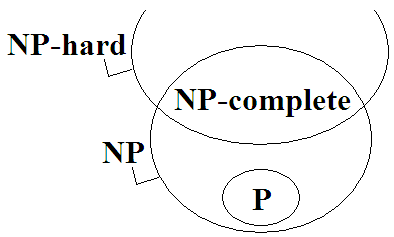
\includegraphics[scale=0.5]{images/NP}
\par\end{center}


\subsection{P 问题}

用多项式时间算法能够计算答案的问题。

\noindent %
\shadowbox{\begin{minipage}[t]{1\columnwidth}%
「找出一群数字当中最大的数字」是P问题。%
\end{minipage}}

P 的全名是 Polynomial time 。通常以「 P 」表示所有 P 问题构成的集合。 


\subsection{NP 问题}

用指数时间算法能够计算答案的问题,同时,用多项式时间算法能够验证答案的问题。

由于 P 问题也可以改用指数时间算法计算答案、当然可以用多项式时间验证答案,故 P 问题都属于 NP 问题。 

\noindent %
\shadowbox{\begin{minipage}[t]{1\columnwidth}%
「找出一张图的一条Hamilton Path」是NP问题。\\


计算答案: 

穷举所有可能的路线,一条一条验证。 

是指数时间算法。\\


验证答案:

给定一条可能的路线,就照着路线走,看看能不能走到每一点。 

是多项式时间算法。 %
\end{minipage}}

\noindent %
\shadowbox{\begin{minipage}[t]{1\columnwidth}%
「找出一张图成本最小的那条Hamilton Path」不是NP问题。\\


计算答案: 

穷举所有可能的路线,一条一条验证。 

是指数时间算法。\\


验证答案: 

就算给定一条可能的路线, 

还是必须穷举所有路线,一条一条验证,才知道哪条路线成本最少。 

是指数时间算法。 %
\end{minipage}}

值得一提的是,每一个 NP 问题,都可以设计出多项式时间算法,转换成另一个 NP 问题。换句话说,所有 NP 问题都可以用多项式时间算法彼此转换。 

NP 的全名是 Non-deterministic Polynomial time ,定义颇复杂,此处省略之。通常以「 NP 」表示所有
NP 问题构成的集合。 


\subsection{NP-complete 问题}

所有 NP 问题当中,最具代表性、层次最高、最难的问题。

NP-complete 问题的各种特例,涵盖了所有 NP 问题。只要有办法解决 NP-complete 问题,就有办法解决 NP 问题。

各个 NP-complete 问题都等价、都一样难,可以用多项式时间算法彼此转换。现今已经找出上百个 NP-complete 问题了。

Complete 的意义为:能够代表整个集合的子集合。举例来说,它就像是一个线性空间( linear space )的基底( basis
)。 

\noindent %
\shadowbox{\begin{minipage}[t]{1\columnwidth}%
「判断一张图是否存在Hamilton Path」已被证明是NP-complete问题。%
\end{minipage}}


\subsection{NP-hard 问题}

用多项式时间算法转换 NP 问题所得到的问题,同时,必须是跟 NP-complete 问题一样难、还要难的问题。 

NP-hard 问题可能是:甲、 NP-complete 问题(是 NP 问题),乙、超出 NP 问题的复杂度,是更难的问题。 

\noindent %
\shadowbox{\begin{minipage}[t]{1\columnwidth}%
「找出一张图成本最小的Hamilton Path」是NP-hard问题。\\


由「找出一张图的一条Hamilton Path」这个NP问题,

用多项式时间把每条边加上成本而得。

而且「找出一张图成本最小的Hamilton Path」至少比NP-complete问题还难。 %
\end{minipage}}


\subsection{P = NP ?}

这是信息科学界的一个悬案。大意是说:到底 NP 问题能不能用多项式时间算法解决呢?如果可以的话,那么 NP 问题就都变成了 P 问题了。这意味着有一些花上几十年几百年算不出答案的问题,变得可以在几分几秒内计算完毕、得到答案。

有一个解决这个悬案的方向是:尝试发明一个多项式时间算法,解决某一个 NP-complete 问题。一旦找到了一个多项式时间算法能够算出某一个
NP-complete 问题的答案,我们可以将此 NP-complete 问题进行特例化得到所有 NP 问题,如此一来,所有 NP
问题就一定可以用多项式时间算法算出答案了。 

很多人声称自己已经成功证明了,但是至今还没有一个让所有人都信服的证明: 

\href{http://www.win.tue.nl/~gwoegi/P-versus-NP.htm}{http://www.win.tue.nl/$\sim$gwoegi/P-versus-NP.htm}


\subsection{介于 P 与 NP-complete 之间的问题}

\href{http://cstheory.stackexchange.com/questions/79/}{http://cstheory.stackexchange.com/questions/79/}


\chapter{Algorithm Design}


\section{Incremental Method}

\begin{flushright}
\textit{不积跬步,无以至千里。不积小流,无以成江海。《荀子》}
\par\end{flushright}


\subsection{Incremental Method}

「递增法」是符合计算机运作特性的方法。计算机执行程序,一次只做一个动作,完成了一件事才做下一件事。当一个问题太大太多时,化整为零、一个一个解决吧! 

合抱之木,生于毫末;九层之台,起于累土;千里之行,始于足下。谨以此句与大家共勉。


\subsection{范例:加总数字}

无论计算机再怎么强,还是得一个一个累加数字。

\begin{center}
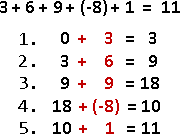
\includegraphics[scale=0.5]{images/Incremental1}
\par\end{center}

\begin{lstlisting}[language={C++},numbers=left,basicstyle={\ttfamily}]
void summation()
{
    int array[5] = {3, 6, 9, -8, 1};
    int sum = 0;
    for (int i=0; i<5; i++)
        sum += array[i];
    cout << "总和是" << sum;
}
\end{lstlisting}


\noindent \rule[0.5ex]{0.75\columnwidth}{1pt}

\begin{lstlisting}[language={C++},numbers=left,basicstyle={\ttfamily}]
int summation(int array[], int n)
{
    int sum = 0;
    for (int i=0; i<n; i++)
        sum += array[i];
    return sum;
}
\end{lstlisting}



\subsection{范例:复制字符串}

无论计算机再怎么强,还是得逐字复制。

\begin{center}
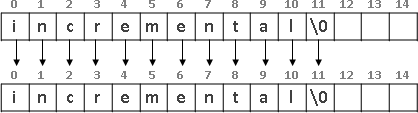
\includegraphics[scale=0.5]{images/Incremental2}
\par\end{center}

\begin{lstlisting}[language={C++},numbers=left,basicstyle={\ttfamily}]
void copy()
{
    char s[15] = "incremental";
    char t[15];

    int i;
    for (i=0; s[i] != '\0'; ++i)
        t[i] = s[i];
    t[i] = '\0';

    cout << "原本字符串" << s;
    cout << "复制之后的字符串" << t;
}
\end{lstlisting}


\noindent \rule[0.5ex]{0.75\columnwidth}{1pt}

\begin{lstlisting}[language={C++},numbers=left,basicstyle={\ttfamily}]
void copy(char* s, char* t)
{
    int i;
    for (i=0; s[i]; ++i)
        t[i] = s[i];
    t[i] = '\0';
}
\end{lstlisting}



\subsection{范例:选择排序法( Selection Sort )}

找到第一小的数字,放在第一个位置;再找到第二小的数字,放在第二个位置。一次找一个数字,如此下去就会把所有数值按照顺序排好了。

\begin{center}
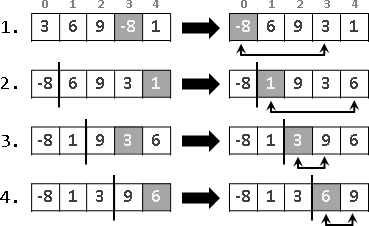
\includegraphics[scale=0.5]{images/Incremental3}
\par\end{center}

\begin{lstlisting}[language={C++},numbers=left,basicstyle={\ttfamily}]
void selection_sort() {
    int array[5] = {3, 6, 9, -8, 1};

    for (int i=0; i<5; ++i)
    {
        // 从尚未排序的数字当中,找到第i小的数值。
        int min_index = i;
        for (int j=i+1; j<5; ++j)
            if (array[j] < array[min_index]) 
                min_index = j;

        // 把第i小的数值,放在第i个位置。
        swap(array[i], array[min_index]);
    }

    // 印出排序结果。
    for (int i=0; i<5; ++i)
        cout << array[i];
}
\end{lstlisting}



\subsection{范例:印出直角三角形}

多字成行,多行成直角三角形。由细微的东西开始,一件一件组起来。

\begin{center}
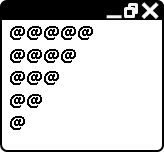
\includegraphics[scale=0.5]{images/Incremental4}
\par\end{center}

\begin{lstlisting}[language={C++},numbers=left,basicstyle={\ttfamily}]
// 多字成行
void print_line(int n)  // n 是一行的长度
{
    for (int i=1; i<=n; i++) cout << '@';
    cout << '\n';
}

// 多行成直角三角形
void print_triangle(int n)  // n 是行数
{
    for (int i=n; i>=1; i--) print_line(i);
}
\end{lstlisting}


\noindent \marginpar{%
\begin{minipage}[t]{10em}%
\begin{shaded}%
UVa \protect\href{http://uva.onlinejudge.org/external/4/488.html}{488}
\protect\href{http://uva.onlinejudge.org/external/100/10038.html}{10038}
\protect\href{http://uva.onlinejudge.org/external/101/10107.html}{10107}
\protect\href{http://uva.onlinejudge.org/external/103/10370.html}{10370}\end{shaded}%
\end{minipage}}


\subsection{范例:人潮最多的时段( Interval Partitioning Problem )}

一群访客参加宴会,我们询问到每一位访客的进场时刻与出场时刻,请问宴会现场挤进最多人的时段。

换个角度想,想象会场门口装着一支监视器。有访客进入,会场就多一人;有访客离开,会场就少一人。如此就很容易统计会场人数。递增的标的是时刻,而不是访客。 

【注:这个技巧在中文网络上昵称为「离散化」。】 

\begin{center}
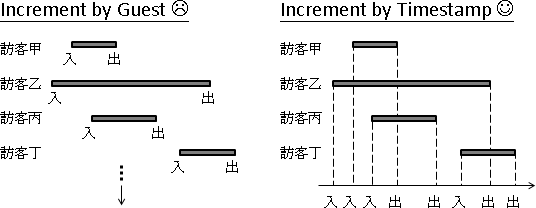
\includegraphics[scale=0.5]{images/Incremental5}
\par\end{center}

\begin{lstlisting}[language={C++},numbers=left,basicstyle={\ttfamily}]
struct Guest {int arrival, leave;} g[10];

bool cmp(const int& i, const int& j)
{
    return abs(i) < abs(j);
}

void maximum_guest()
{
    vector<int> time;
    for (int i=0; i<10; ++i)
    {
        time.push_back(+g[i].arrival);
        time.push_back(-g[i].leave);
    }

    sort(time.begin(), time.end(), cmp);

    int n = 0, maximum = 0;
    for (int i=0; i<time.size(); ++i)
    {
        if (time[i] >= 0)
            n++;
        else
            n--;

        maximum = max(maximum, n);
    }
    cout << "人潮最多的时段有" << maximum << "人";
}
\end{lstlisting}


此处仅找出人数。找出人潮最多的时段,就留给各位自行尝试吧。

\noindent \marginpar{%
\begin{minipage}[t]{10em}%
\begin{shaded}%
UVa \protect\href{http://uva.onlinejudge.org/external/6/688.html}{688}
\protect\href{http://uva.onlinejudge.org/external/9/972.html}{972}
\protect\href{http://uva.onlinejudge.org/external/106/10613.html}{10613}
\protect\href{http://uva.onlinejudge.org/external/105/10585.html}{10585}
\protect\href{http://uva.onlinejudge.org/external/109/10963.html}{10963}

UVa \protect\href{http://uva.onlinejudge.org/external/3/308.html}{308}
\protect\href{http://uva.onlinejudge.org/external/8/837.html}{837}\end{shaded}%
\end{minipage}}


\subsection{范例:储存坐标}

递增的标的,主为点,次为坐标轴。

\begin{lstlisting}[language={C++},numbers=left,basicstyle={\ttfamily}]
struct Point {float x, y;} p[5] = 
{
    {0, 1}, {1, 2}, {3, 0}, {2, 2}, {3, 1}
}; 
\end{lstlisting}


递增的标的,主为坐标轴,次为点。

\begin{center}
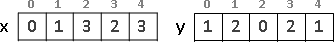
\includegraphics[scale=0.5]{images/Incremental7}
\par\end{center}

\begin{lstlisting}[language={C++},numbers=left,basicstyle={\ttfamily}]
float x[5] = {0, 1, 3, 2, 3};
float y[5] = {1, 2, 0, 2, 1};
\end{lstlisting}



\subsection{范例:印出转换成小写的字符串}

\begin{center}
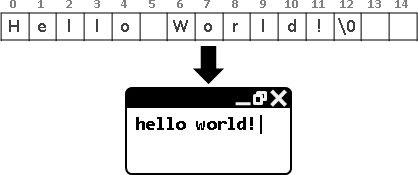
\includegraphics[scale=0.5]{images/Incremental8}
\par\end{center}

有需要改变的,只有大写字母──如果是大写字母,就转换成小写字母并且印出;如果不是大写字母,就直接印出。

\begin{lstlisting}[language={C++},numbers=left,basicstyle={\ttfamily}]
void print_lowercase()
{
    char s[15] = "Hello World!";

    char t[15];

    // 第一波:复制字符串
    for (int i=0; s[i]; i++)
        t[i] = s[i];

    // 第二波:换成小写
    for (int i=0; s[i]; i++)
        if (t[i] >= 'A' && t[i] <= 'Z')
            t[i] = t[i] - 'A' + 'a';

    // 第三波:印出字符串
    cout << t;
}
\end{lstlisting}


\noindent \rule[0.5ex]{0.75\columnwidth}{1pt}

\begin{lstlisting}[language={C++},numbers=left,basicstyle={\ttfamily}]
void print_lowercase()
{
    char s[15] = "Hello World!";

    char t[15];

    // 每一波的程序代码可以自行包装成为函数,
    // 亦可套用内建函数库。
    my_copy(s, t);      // 复制字符串
    my_lowercase(t);    // 换成小写
    cout << t;          // 印出字符串
}
\end{lstlisting}


第一种解法称作 one-pass ,数据只会读取一遍。读取数据的同时,也一口气处理掉所有事情。

第二种解法称作 multi-pass ,数据会重复读取许多遍。所有事情划分成数个阶段,逐步处理,每个阶段只专心处理一件事情。

one-pass 的优点是:程序代码简短、执行时间也短。缺点是:程序代码不易编修。

multi-pass 的优点是:程序代码一目了然,容易编修、测试、除错;程序代码可以包装成为函数,也有机会套用内建函数库。缺点是:需要额外的暂存内存。

这两种方式各有利弊。程序员必须自行取舍。 


\subsection{范例:对调数字}

利用一个变量,暂存其中一个数字,以便对调。

\begin{center}
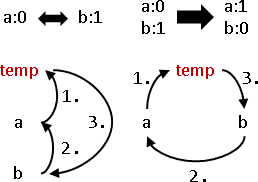
\includegraphics[scale=0.5]{images/Incremental9}
\par\end{center}

\begin{lstlisting}[language={C++},numbers=left,basicstyle={\ttfamily}]
void swap_int()
{
    int a = 0, b = 1;

    // 交换a与b
    int temp = a;
    a = b;
    b = temp;

    cout << a << ' ' << b;
}
\end{lstlisting}


\noindent \rule[0.5ex]{0.75\columnwidth}{1pt}

\begin{lstlisting}[language={C++},numbers=left,basicstyle={\ttfamily}]
void swap_int(int& a, int& b)
{
    int temp = a;
    a = b;
    b = temp;
}
\end{lstlisting}



\subsection{范例:对调数组}

节省内存的方法:采用递增法,逐一对调数字。

\begin{center}
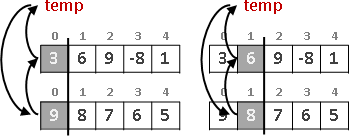
\includegraphics[scale=0.5]{images/Incremental10}
\par\end{center}

\begin{lstlisting}[language={C++},numbers=left,basicstyle={\ttfamily}]
void swap_int_array()
{
    int a[5] = {3, 6, 9, -8, 1};
    int b[5] = {9, 8, 7, 6, 5};

    // one-pass
    for (int i=0; i<5; ++i)
    {
        int temp = a[i];
        a[i] = b[i];
        b[i] = temp;
    }
}
\end{lstlisting}


\noindent 浪费内存的方法:建立一个数组,暂存其中一个数组。

\begin{center}
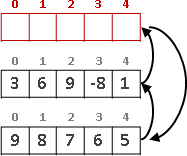
\includegraphics[scale=0.5]{images/Incremental11}
\par\end{center}

\begin{lstlisting}[language={C++},numbers=left,basicstyle={\ttfamily}]
void swap_int_array()
{
    int a[5] = {3, 6, 9, -8, 1};
    int b[5] = {9, 8, 7, 6, 5};

    // multi-pass
    int temp[5];
    for (int i=0; i<5; ++i) temp[i] = a[i];
    for (int i=0; i<5; ++i) a[i] = b[i];
    for (int i=0; i<5; ++i) b[i] = temp[i];
}
\end{lstlisting}


\noindent \rule[0.5ex]{0.75\columnwidth}{1pt}

\begin{lstlisting}[language={C++},numbers=left,basicstyle={\ttfamily}]
void swap_int_array()
{
    int a[5] = {3, 6, 9, -8, 1};
    int b[5] = {9, 8, 7, 6, 5};

    // multi-pass
    int temp[5];
    my_copy(a, temp);
    my_copy(b, a);
    my_copy(temp, b);
}
\end{lstlisting}



\section{Memoization}

\begin{flushright}
\textit{惟事事,乃其有备,有备无患。《书经》}
\par\end{flushright}


\subsection{Memoization}

「记忆法」是符合计算机运作特性的方法。计算机拥有大量储存空间。只要将计算过的数值,储存于内存,往后就能直接使用内存储存的数据,不必再浪费时间重复计算一遍。

\noindent %
\shadowbox{\begin{minipage}[t]{1\columnwidth}%
Memoization(Tabulation)

算法执行过程之中,实时更新数值,储存于内存。 

例如堆栈的大小。\\


Preprocessing(Precalculation)

算法开始之时,预先计算数值,储存于内存。

例如圆周率、字符串的长度、质数的表格。 %
\end{minipage}}

如果要储存大量的、同性质的数值,我们可以将这些数值整理成一个表格(通常是数组),以方便查阅──称作「查询表 lookup table
」。例如质数表便是一个「查询表」。


\subsection{范例:数组大小}

使用一个变量,纪录数据数量,以便迅速地增加数据。

\begin{center}
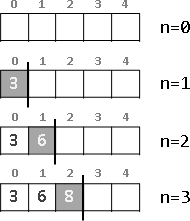
\includegraphics[scale=0.5]{images/Memorization1}
\par\end{center}

\begin{lstlisting}[language={C++},numbers=left,basicstyle={\ttfamily}]
void array_size()
{
    int array[100];
    int n = 0;      // 使用一个变量,纪录数据数量。
    array[n++] = 3; // 以便迅速地增加数据。
    array[n++] = 6;
    array[n++] = 9;
    cout << n;
}
\end{lstlisting}


C++ 程序语言的标准函数库的 stack ,事实上也额外隐含了一个变量,纪录数据数量。当堆栈塞入数据、弹出数据的时候,也就是调用
push 函数、调用 pop 函数的时候,就默默更新数据数量。

\begin{lstlisting}[language={C++},numbers=left,basicstyle={\ttfamily}]
void stack_size()
{
    stack<int> s;       // C++ STL <stack>
    s.push(1);          // 默默地n++
    s.pop();            // 默默地--n
    cout << s.size();   // 把n印出来
}
\end{lstlisting}



\subsection{范例:加总数字}

利用一个变量,累计数字的总和。

\begin{center}
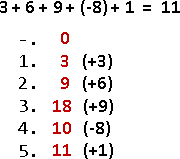
\includegraphics[scale=0.5]{images/Memorization2}
\par\end{center}

\begin{lstlisting}[language={C++},numbers=left,basicstyle={\ttfamily}]
void summation()
{
    int array[5] = {3, 6, 9, -8, 1};
    int sum = 0;
    for (int i=0; i<5; i++)
        sum += array[i];
    cout << "总和是" << sum;
}
\end{lstlisting}


\noindent \rule[0.5ex]{0.75\columnwidth}{1pt}

\begin{lstlisting}[language={C++},numbers=left,basicstyle={\ttfamily}]
int summation(int array[], int n)
{
    int sum = 0;
    for (int i=0; i<n; i++)
        sum += array[i];
    return sum;
}
\end{lstlisting}



\subsection{范例:统计字母数量}

建立 26 格的数组,让字母 a 到 z 依序对应数组的每一格,作为 lookup table 。一边读取字符串,一边累计字母出现次数。

\begin{center}
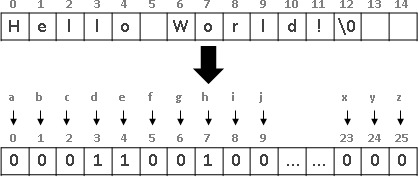
\includegraphics[scale=0.5]{images/Memorization3}
\par\end{center}

\begin{lstlisting}[language={C++},numbers=left,basicstyle={\ttfamily}]
void count_letter()
{
    char s[15] = "Hello World!";
    int c[26] = {0};

    // 字母一律换成小写
    for (int i=0; s[i]; i++)
        if (s[i] >= 'A' && s[i] <= 'Z')
            s[i] = s[i] - 'A' + 'a';

    // 统计字母数量
    for (int i=0; s[i]; i++)
        if (s[i] >= 'a' && s[i] <= 'z')
            c[s[i] - 'a']++;

    // 印出统计结果
    for (int i=0; i<26; i++)
        cout << char('a'+i) << ':' << c[i] << '\n';
}
\end{lstlisting}


\noindent \marginpar{%
\begin{minipage}[t]{10em}%
\begin{shaded}%
UVa \protect\href{http://uva.onlinejudge.org/external/102/10260.html}{10260}
\protect\href{http://uva.onlinejudge.org/external/100/10082.html}{10082}
\protect\href{http://uva.onlinejudge.org/external/102/10222.html}{10222}
\protect\href{}{12626}\end{shaded}%
\end{minipage}}


\subsection{范例:统计数字数量}

当数字范围太大,无法建立那么大的数组,可以改用 hash table 、 binary search tree 等等数据结构作为 lookup
table 。

\begin{center}
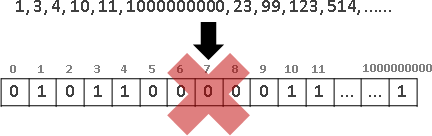
\includegraphics[scale=0.5]{images/Memorization4}
\par\end{center}

\begin{lstlisting}[language={C++},numbers=left,basicstyle={\ttfamily}]
void count_number()
{
    int array[10] =
    {
        1, 3, 4, 10, 11,
        1000000000, 23, 99, 123, 514
    };
//  int c[1000000000] = {0};
    map<int, int> c;   // binary search tree

    // 统计数字数量
    for (int i=0; i<10; i++)
        c[array[i]]++;

    // 印出统计结果
    for (auto i=c.begin(); i!=c.end(); ++i)
        cout << i->first << ':' << i->second << '\n';
}
\end{lstlisting}


\noindent \marginpar{%
\begin{minipage}[t]{10em}%
\begin{shaded}%
UVa \protect\href{http://uva.onlinejudge.org/external/115/11572.html}{11572}
\protect\href{http://uva.onlinejudge.org/external/1/141.html}{141}\end{shaded}%
\end{minipage}}


\subsection{范例:求 1 到 n 的全部整数的立方和, n 的范围由 1 到 10 。}

\begin{center}
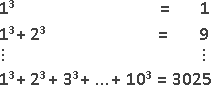
\includegraphics[scale=0.5]{images/Memorization5}
\par\end{center}

以直接的方式,累加每个立方数。(尽管这个问题有公式解,但是为了方便举例,所以这里不采用公式解。)

\begin{lstlisting}[language={C++},numbers=left,basicstyle={\ttfamily}]
int sum_of_cubes(int n)
{
    int sum = 0;
    for (int i=1; i<=n; i++)
        sum += i * i * i;
    return sum;
}

void print_sum_of_cubes()
{
    int n;
    while (cin >> n && n > 0)
        cout << sum_of_cubes(n);
}
\end{lstlisting}


使用 Memoization 。建立 11 格的数组,每一格依序对应 0 到 10 的立方数,作为 lookup table 。一旦计算完毕,就储存至表格;往后就直接读取表格,不需重复计算。

\begin{lstlisting}[language={C++},numbers=left,basicstyle={\ttfamily}]
int sum_of_cubes(int n)
{
    // 其值为 0 表示没有存入答案
    static int answer[10 + 1] = {};

    // 如果已经计算过,就直接读取表格的答案。
    if (answer[n] != 0) return answer[n];

    // 如果不曾计算过,就计算一遍,储存答案。
    int sum = 0;
    for (int i=1; i<=n; i++)
        sum += i * i * i;
    return answer[n] = sum;
}

void print_sum_of_cubes()
{
    int n;
    while (cin >> n && n > 0)
        cout << sum_of_cubes(n);
}
\end{lstlisting}


使用 Preprocessing 。

\begin{lstlisting}[language={C++},numbers=left,basicstyle={\ttfamily}]
void print_sum_of_cubes()
{
    // 预先建立立方数表格
    int cube[10 + 1];
    for (int i=1; i<=10; ++i)
        cube[i] = i * i * i;

    int n;
    while (cin >> n && n > 0)
    {
        // 直接读取表格的立方数
        int sum = 0;
        for (int i=1; i<=n; ++i)
            sum += cube[i];
        cout << sum;
    }
}
\end{lstlisting}


Preprocessing 当然也可以直接算答案啦。

\begin{lstlisting}[language={C++},numbers=left,basicstyle={\ttfamily}]
int sum_of_cubes(int n)
{
    int sum = 0;
    for (int i=1; i<=n; i++)
        sum += i * i * i;
    return sum;
}

void print_sum_of_cubes()
{
    // 预先计算所有答案
    int answer[10 + 1];
    for (int i=1; i<=10; ++i)
        answer[i] = sum_of_cubes(i);

    // 直接读取表格的答案
    int n;
    while (cin >> n && n > 0)
        cout << answer[n];
}
\end{lstlisting}


最后是 Preprocessing 的极致。

\begin{lstlisting}[language={C++},numbers=left,basicstyle={\ttfamily}]
void print_sum_of_cubes()
{
    // 预先计算答案,写死在程序代码里面。
    int answer[10 + 1] =
    {
        0, 1, 9, 36, 100, 225,
        441, 784, 1296, 2025, 3025
    };

    // 直接读取表格的答案
    int n;
    while (cin >> n && n > 0)
        cout << answer[n];
}
\end{lstlisting}


\noindent \marginpar{%
\begin{minipage}[t]{10em}%
\begin{shaded}%
UVa \protect\href{http://uva.onlinejudge.org/external/107/10738.html}{10738}
\protect\href{http://uva.onlinejudge.org/external/108/10894.html}{10894}\end{shaded}%
\end{minipage}}


\subsection{范例:印出方框}

建立二维数组:数组的格子,依序对应窗口的文字。

\begin{center}
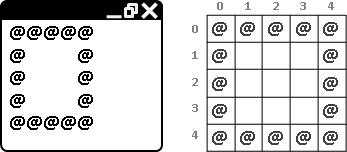
\includegraphics[scale=0.5]{images/Memorization6}
\par\end{center}

不直接印出方框,而是间接填至数组。不必数空格键,只需两条水平线和两条垂直线。

\begin{lstlisting}[language={C++},numbers=left,basicstyle={\ttfamily}]
void print_square_border()
{
    // 建立内存
    char array[5][5];

    // 预先填入空格键
    for (int i=0; i<5; ++i)
        for (int j=0; j<5; ++j)
            array[i][j] = ' ';

    // 填入方框:两条水平线、两条垂直线
    // 即便相互重叠也无所谓
    for (int i=0; i<5; ++i) array[0][i] = '@';
    for (int i=0; i<5; ++i) array[4][i] = '@';
    for (int i=0; i<5; ++i) array[i][0] = '@';
    for (int i=0; i<5; ++i) array[i][4] = '@';

    // 印出方框
    for (int i=0; i<5; ++i)
    {
        for (int j=0; j<5; ++j)
            cout << array[i][j];
        cout << '\n';
    }
}
\end{lstlisting}


\noindent \marginpar{%
\begin{minipage}[t]{10em}%
\begin{shaded}%
UVa \protect\href{http://uva.onlinejudge.org/external/1/105.html}{105}
\protect\href{http://uva.onlinejudge.org/external/7/706.html}{706}\end{shaded}%
\end{minipage}}


\subsection{范例:拆开循环( Loop Unrolling )}

\begin{center}
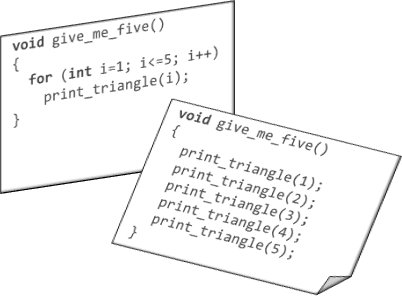
\includegraphics[scale=0.5]{images/Memorization7}
\par\end{center}

循环语法的功能是:一段指令,重复实施数次,但是每次都稍微变动一点点。

事实上,我们可以反璞归真,拆开循环,还原成数行指令。如此一来,就节省了循环每次累加变量的时间,也节省了循环每次判断结束条件的时间。

拆开循环是一种 Preprocessing ,预先计算循环变量、预先计算循环结束条件。

拆开循环之后,虽然提高了程序的执行速度,但是降低了程序可读性。程序员必须自行取舍。 


\section{Enumeration}

\begin{flushright}
\textit{愚者千虑,必有一得。《史记》}
\par\end{flushright}


\subsection{Enumeration}

「枚举法」利用了计算机无与伦比的计算速度。找到不确定的变量,枚举所有可能性,逐一判断正确性。

\noindent %
\shadowbox{\begin{minipage}[t]{1\columnwidth}%
Enumerate

一笔一笔列出所有数据。

对应到程序语言的for。\\


Search

浏览所有数据,找出需要的部份。

对应到程序语言的for加if。 %
\end{minipage}}

收集充分信息,就能解决问题。

\begin{center}
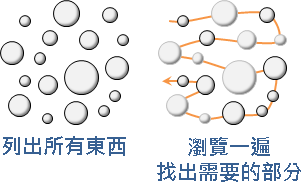
\includegraphics[scale=0.5]{images/Enumeration1}
\par\end{center}


\subsection{范例:枚举一百个平方数}

采用直接法:依序枚举数字 1 到 100 ;枚举过程当中,将数字平方得到平方数。

\begin{center}
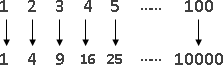
\includegraphics[scale=0.5]{images/Enumeration2}
\par\end{center}

\begin{lstlisting}[language={C++},numbers=left,basicstyle={\ttfamily}]
void generate_squares()
{
    for (int i=1; i<=100; i++)
        cout << i*i << "是平方数";
}
\end{lstlisting}


采用试误法:依序枚举数字 1 到 $\infty$ ;枚举过程当中,判断数字是不是平方数。

\begin{center}
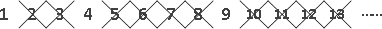
\includegraphics[scale=0.5]{images/Enumeration3}
\par\end{center}

\begin{lstlisting}[language={C++},numbers=left,basicstyle={\ttfamily}]
void generate_squares()
{
    for (int i=1; i<=100*100; i++)
    {
        int sqrt_i = sqrt(i);
        if (sqrt_i * sqrt_i == i)
            cout << i << "是平方数";
    }
}
\end{lstlisting}



\subsection{范例:寻找数组里的最小值}

由小到大枚举数组索引值,逐一比较数组元素。

\begin{center}
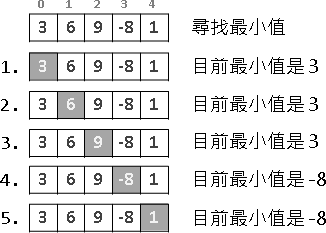
\includegraphics[scale=0.5]{images/Enumeration4}
\par\end{center}

\begin{lstlisting}[language={C++},numbers=left,basicstyle={\ttfamily}]
void find_minimum()
{
    int array[5] = {3, 6, 9, -8, 1};

    int min = 2147483647;
    for (int i=0; i<5; i++) // 枚举索引值
        if (array[i] < min) // 比较元素
            min = array[i]; // 随时纪录最小值

    cout << "最小的数字是" << min;
}
\end{lstlisting}


\noindent \rule[0.5ex]{0.75\columnwidth}{1pt}

\begin{lstlisting}[language={C++},numbers=left,basicstyle={\ttfamily}]
int find_minimum(int array[], int n)
{
    int min = 2147483647;
    for (int i=0; i<n; i++) // 枚举索引值
        if (array[i] < min) // 比较元素
            min = array[i]; // 随时纪录最小值
    return min;
}
\end{lstlisting}



\subsection{范例:寻找数组里的特定数字}

找到所有特定数字:浏览一遍所有数字。

\begin{center}
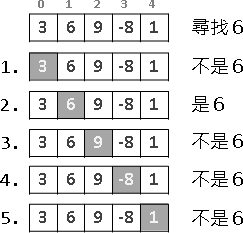
\includegraphics[scale=0.5]{images/Enumeration5}
\par\end{center}

\begin{lstlisting}[language={C++},numbers=left,basicstyle={\ttfamily}]
void find_all_number()
{
    int array[5] = {3, 6, 9, -8, 1};

    for (int i=0; i<5; i++) // 枚举
        if (array[i] == 6)  // 搜寻
            cout << i << ':' << array[i] << '\n';
}
\end{lstlisting}


找到其中一个特定数字:一旦找到,立即停止浏览,以节省时间。

\begin{center}
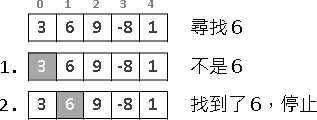
\includegraphics[scale=0.5]{images/Enumeration6}
\par\end{center}

\begin{lstlisting}[language={C++},numbers=left,basicstyle={\ttfamily}]
bool find_number()
{
    int array[5] = {3, 6, 9, -8, 1};

    for (int i=0; i<5; i++) // 枚举
        if (array[i] == 6)  // 搜寻
        {
            cout << i << ':' << array[i];
            return true;
        }
    return false;
}
\end{lstlisting}


\noindent \rule[0.5ex]{0.75\columnwidth}{1pt}

\begin{lstlisting}[language={C++},numbers=left,basicstyle={\ttfamily}]
int find_number(int array[i], int n, int num)
{
    for (int i=0; i<n; i++)
        if (array[i] == num)
            return i;
    return -1;
}
\end{lstlisting}



\subsection{范例:寻找二维数组里的特定数字}

\begin{center}
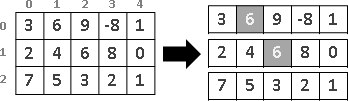
\includegraphics[scale=0.5]{images/Enumeration7}
\par\end{center}

多个元素成为一个横条、多个横条成为一个数组。内层先枚举元素,外层再枚举横条,就能枚举所有元素。

方才是由内而外、由小到大进行思考,其实也可以由外而内、由大到小进行思考:外层先枚举每一个横条,内层再枚举一个横条的每一个元素,就能枚举所有元素。 

\begin{lstlisting}[language={C++},numbers=left,basicstyle={\ttfamily}]
bool find(int n)
{
    int array[3][5] =
    {
        {3, 6, 9, -8, 1},
        {2, 4, 6, 8, 10},
        {11, 7, 5, 3, 2}
    };

    // 外层枚举每一个横条
    for (int i=0; i<3; i++)
        // 内层枚举一个横条的每一个元素
        for (int j=0; j<5; j++)
            // 就能枚举所有元素
            if (array[i][j] == n)
                return true;
    return false;
}
\end{lstlisting}


此处再介绍一种特别的思考方式:第一层枚举每一个横条,第二层枚举每一个直条,就能枚举所有直条与横条的交错之处。

虽然前后两个思考方式完全不同,但是前后两支程序代码却完全相同。 

\begin{lstlisting}[language={C++},numbers=left,basicstyle={\ttfamily}]
bool find(int n)
{
    int array[3][5] =
    {
        {3, 6, 9, -8, 1},
        {2, 4, 6, 8, 10},
        {11, 7, 5, 3, 2}
    };

    // 第一层枚举每一个横条
    for (int i=0; i<3; i++)
        // 第二层枚举每一个直条
        for (int j=0; j<5; j++)
            // 就能枚举所有横条与直条交错之处
            if (array[i][j] == n)
                return true;
    return false;
}
\end{lstlisting}



\subsection{范例:平面上距离最近的两个点( Closest Pair Problem )}

\begin{center}
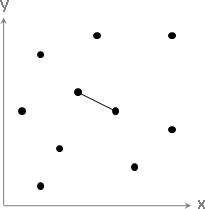
\includegraphics[scale=0.5]{images/Enumeration8}
\par\end{center}

第一层枚举第一个点,第二层枚举第二个点。为了避免重复枚举相同的一对点,第二层只枚举索引值更高的点。

\begin{lstlisting}[language={C++},numbers=left,basicstyle={\ttfamily}]
void closest_pair()
{
    float point[10][2] =
    {
        {3, 3}, {1, 5}, {4, 6}, {2, 8}, {9, 9},
        {2, 1}, {7, 2}, {6, 5}, {9, 4}, {5, 9}
    };

    // 距离最近的两个点的距离
    float d = 1e9;

    // 枚举第一点
    for (int i=0; i<10; i++)
        // 枚举第二点
        for (int j=i+1; j<10; j++)
        {
            // 计算第一点到第二点的距离
            float dx = point[i][0] - point[j][0];
            float dy = point[i][1] - point[j][1];
            float dij = sqrt(dx * dx + dy * dy);

            // 纪录最短的距离
            if (dij < d) d = dij;
        }
    cout << "距离是" << d;
}
\end{lstlisting}


可以把计算距离的程序代码,抽离出来成为一个函数。好处是程序代码变得清爽许多,增加程序代码可读性。坏处是大量调用函数,导致执行速度变慢。

\begin{lstlisting}[language={C++},numbers=left,basicstyle={\ttfamily}]
struct Point {float x, y;};

// 计算两点之间的距离
float dist(Point& a, Point& b)
{
    float dx = a.x - b.x;
    float dy = a.y - b.y;
    return sqrt(dx * dx + dy * dy);
}

void closest_pair()
{
    Point point[10] =
    {
        {3, 3}, {1, 5}, {4, 6}, {2, 8}, {9, 9},
        {2, 1}, {7, 2}, {6, 5}, {9, 4}, {5, 9}
    };

    float d = 1e9;
    for (int i=0; i<10; i++)
        for (int j=i+1; j<10; j++)
            // 纪录最短的距离
            d = min(d, dist(point[i], point[j]));

    cout << "距离是" << d;
}
\end{lstlisting}


鱼与熊掌不可兼得,这两种程序代码各有优缺点,没有绝对的好坏。程序员必须自行取舍。


\subsection{范例:字符串匹配( String Matching )}

从长字符串之中,找到短字符串的出现位置。

\begin{center}
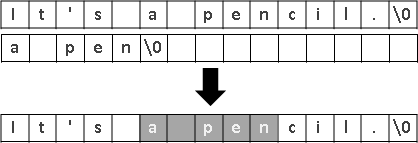
\includegraphics[scale=0.5]{images/Enumeration9}
\par\end{center}

第一层先枚举所有可以匹配的位置,第二层再枚举所有需要匹配的字符。

\begin{lstlisting}[language={C++},numbers=left,basicstyle={\ttfamily}]
void string_matching()
{
    char text[15] = "It's a pencil.";
    char pattern[6] = "a pen";

    // 枚举所有可以匹配的位置
    for (int i=0; i<14; i++)
    {
        // 枚举所有需要匹配的字符
        bool match = true;
        for (int j=0; j<5; j++)
            if (text[i+j] != pattern[j])
                match = false;

        if (match)
            cout << "短字符串出现在第" << i << "个字符";
    }
}
\end{lstlisting}


因为短字符串不会超出长字符串末段,所以第一层枚举范围可以再略微缩小。

因为只要一个相异字符,就足以表明匹配位置错误,所以第二层的枚举过程可以提早结束。 

\begin{lstlisting}[language={C++},numbers=left,basicstyle={\ttfamily}]
void string_matching()
{
    char text[15] = "It's a pencil.";
    char pattern[6] = "a pen";

    // 仔细估量枚举范围
    for (int i=0; i<14-6+1; i++)
    {
        bool match = true;
        for (int j=0; j<5; j++)
            if (text[i+j] != pattern[j])
            {
                match = false;
                break;
            }

        if (match)
            cout << "短字符串出现在第" << i << "个字符";
    }
}
\end{lstlisting}



\subsection{范例:统计字母数量}

\begin{center}
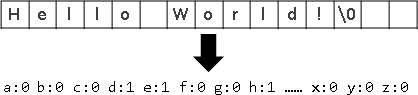
\includegraphics[scale=0.5]{images/Enumeration10}
\par\end{center}

第一层先枚举 26 种英文字母,第二层再枚举字符串的所有字符,计算一种字母的数量。

\begin{lstlisting}[language={C++},numbers=left,basicstyle={\ttfamily}]
void count_letter()
{
    char s[15] = "Hello World!";

    // 字母统一换成小写
    for (int i=0; s[i]; i++)
        if (s[i] >= 'A' && s[i] <= 'Z')
            s[i] = s[i] - 'A' + 'a';

    // 枚举26种英文字母
    for (int i=0; i<26; i++)
    {
        // 枚举字符串的所有字符
        int c = 0;
        for (int j=0; s[j]; j++)
            if (s[j] == i)
                c++;

        // 印出一种字母的数量
        cout << (char)i << ':' << c;
    }
}
\end{lstlisting}


先前曾经介绍过统计字母数量的范例。先前范例当中,虽然耗费内存空间,但是执行速度快──简单来说就是空间大、时间小。此处范例当中,则是空间小,时间大,恰恰相反。这两种方式各有优缺点,程序员必须自行取舍。


\subsection{范例:反转字符串}

\begin{center}
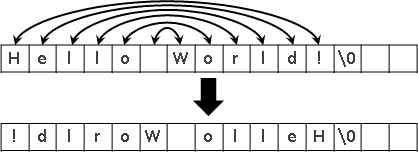
\includegraphics[scale=0.5]{images/Enumeration11}
\par\end{center}

两个枚举,一个从头到尾,一个从尾到头,步调相同,逐步对调字符。虽然是两个枚举,却只有一个循环。

\begin{lstlisting}[language={C++},numbers=left,basicstyle={\ttfamily}]
void reverse_string()
{
    char s[15] = "Hello World!";

    // 两个枚举,一个从头到尾,一个从尾到头。
    for (int i=0, j=12; i<j; i++, j--)
        swap(s[i], s[j]);

    cout << "反转之后的字符串是" << s;
}
\end{lstlisting}


\noindent \rule[0.5ex]{0.75\columnwidth}{1pt}

\begin{lstlisting}[language={C++},numbers=left,basicstyle={\ttfamily}]
void reverse(char* s)
{
    int n = strlen(s);
    for (int i=0; i<n/2; i++)
        swap(s[i], s[n-1-i]);
}
\end{lstlisting}



\subsection{范例:寻找总和为 10 的区间}

假设数组元素只有正数。

\begin{center}
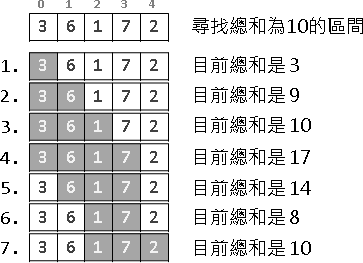
\includegraphics[scale=0.5]{images/Enumeration12}
\par\end{center}

两个枚举,枚举区间左端以及枚举区间右端,都是从头到尾,保持一左一右,视情况轮流枚举。虽然是两个枚举,却只有一个循环。

\begin{lstlisting}[language={C++},numbers=left,basicstyle={\ttfamily}]
void find_interval()
{
    int array[5] = {3, 6, 1, 7, 2};

    int sum = 0;
    for (int i=0, j=-1; j<5; )  // 枚举区间[i, j]
    {
        if (sum > 10)
        {
            // 总和太大,区间左端往右缩短。
            sum -= array[i];
            i++;
        }
        else if (sum < 10)
        {
            // 总和太小,区间右端往右伸长。
            j++;
            sum += array[j];
        }
        else if (sum == 10)
        {
            // 总和刚好,
            // 区间左端往右缩短,
            // 亦得区间右端往右伸长。
            // 任选一种皆可。
//          sum -= array[i];
//          i++;
            j++;
            sum += array[j];
        }

         if (sum == 100)
            cout << '[' << i << ',' << j << ']';
    }
}
\end{lstlisting}


\noindent \rule[0.5ex]{0.75\columnwidth}{1pt}

\begin{lstlisting}[language={C++},numbers=left,basicstyle={\ttfamily}]
void find_interval(int array[], int n, int num)
{     int sum = 0;
    for (int i=0, j=0; j<=n; )  // 枚举区间[i, j)
    {
        if (sum > num)
            sum -= array[i++];
        else
            sum += array[j++];

        if (sum == num)
            cout << '[' << i << ',' << j-1 << ']';
    }
}
\end{lstlisting}


读者可以想想看:数组元素若有零、有负数,是否要调整枚举方式?

\noindent \marginpar{%
\begin{minipage}[t]{10em}%
\begin{shaded}%
UVa \protect\href{http://uva.onlinejudge.org/external/9/972.html}{972}
\protect\href{http://uva.onlinejudge.org/external/104/10464.html}{10464}
\protect\href{http://uva.onlinejudge.org/external/115/11536.html}{11536}
\protect\href{http://uva.onlinejudge.org/external/115/11572.html}{11572}\end{shaded}%
\end{minipage}}


\subsection{范例:寻找数组之中的最小值,数组已经由小到大排序}

找到其中一个最小值:经常整理房间,寻找东西就快;预先排序数据,搜寻速度就快。

\begin{center}
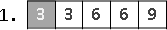
\includegraphics[scale=0.5]{images/Enumeration13}
\par\end{center}

\begin{lstlisting}[language={C++},numbers=left,basicstyle={\ttfamily}]
void find_minimum()
{
    int array[5] = {3, 3, 6, 6, 9};
    cout << "最小的数字是" << array[0];
}
\end{lstlisting}


找到所有最小值:读者请自行尝试。


\subsection{范例:寻找数组之中的特定数字,数组已经由小到大排序}

找到其中一个特定数字:首先找到数组中央的数字,依其数字大小,继续搜寻左半段或者右半段。

\begin{center}
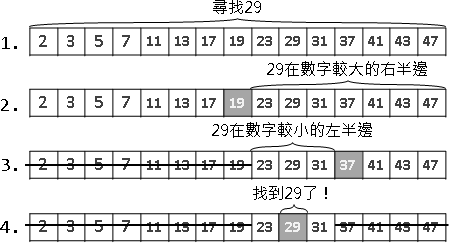
\includegraphics[scale=0.5]{images/Enumeration14}
\par\end{center}

\begin{lstlisting}[language={C++},numbers=left,basicstyle={\ttfamily}]
void find_number()
{
    int array[15] =
    {
        2, 3, 5, 7, 11,
        13, 17, 19, 23, 29,
        31, 37, 41, 43, 47
    };

    int left = 0, right = 15-1;
    while (left < right)
    {
        int mid = (left + right) / 2;
        if (array[mid] < 29)
            left = mid + 1;     // 继续搜寻剩下的右半段
        else if (array[mid] > 29)
            right = mid - 1;    // 继续搜寻剩下的左半段
        else if (array[mid] == 29)
        {
            // 找到了其中一个数字
            cout << mid << ':' << array[mid];
            return;
        }
    }
}
\end{lstlisting}


找到所有特定数字:读者请自行尝试。


\subsection{范例:平面上距离最近的两个点( Closest Pair Problem )}

\begin{center}
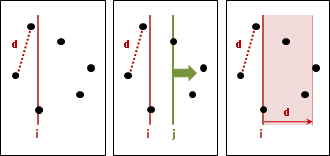
\includegraphics[scale=0.5]{images/Enumeration15}
\par\end{center}

找到距离最近的其中一对点:预先依照 X 坐标排序所有点,搜寻得以略过大量情况。

\begin{lstlisting}[language={C++},numbers=left,basicstyle={\ttfamily}]
struct Point {float x, y;};

// 计算两点之间的距离
float dist(Point& a, Point& b)
{
    float dx = a.x - b.x;
    float dy = a.y - b.y;
    return sqrt(dx * dx + dy * dy);
}

bool cmp(const Point& i, const Point& j)
{
    return i.x < j.x;
}

void closest_pair()
{
    Point point[10] =
    {
        {3, 3}, {1, 5}, {4, 6}, {2, 8}, {9, 9},
        {2, 1}, {7, 2}, {6, 5}, {9, 4}, {5, 9}
    };

    // 依照X坐标排序所有点
    sort(point, point+10, cmp);

    float d = 1e9;
    for (int i=0; i<10; i++)
        for (int j=i+1; j<10; j++)
        {
            // 两个点的X坐标已经相距太远,直接略过,
            // 继续枚举下一个左端点。
            if (p[j].x - p[i].x > d) break;
            d = min(d, dist(point[i], point[j]));
        }

    cout << "距离是" << d;
}
\end{lstlisting}


找到距离最近的每一对点:读者请自行尝试。


\subsection{范例:英文单字从单数变复数}

枚举各种情况,写成大量判断式。

\begin{center}
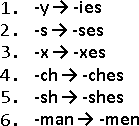
\includegraphics[scale=0.5]{images/Enumeration16}
\par\end{center}

\begin{lstlisting}[language={C++},numbers=left,basicstyle={\ttfamily}]
void plural(string s)
{
    int n = s.length();
    if (s.back() == 'y')
        cout << s.substr(0, n-1) << "ies";
    else if (s.back() == 's' || s.back() == 'x')
        cout << s << "es";
    else if (s.substr(n-2) == "sh" || s.substr(n-2) == "ch")
        cout << s << "es";
    else if (s.substr(n-3) == "man")
        cout << s.substr(0, n-3) << "men";
    else
        cout << s << 's';
}
\end{lstlisting}



\subsection{范例:小画家倒墨水( Flood Fill Algorithm )}

计算机图片可以想成是一张方格纸,每个方格都填着一种颜色。现在要实现小画家倒墨水的功能:以某一格为起点,只要相邻方格颜色一样,就染成同一个颜色。

\begin{center}
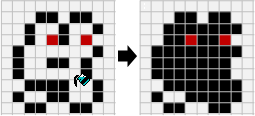
\includegraphics[scale=0.5]{images/Enumeration17}
\par\end{center}

运用大量指令,枚举上下左右四个方向;运用递归,枚举相邻同色方格。 

必须避免已经枚举过的方格又重复枚举,否则程序在有生之年都不会结束。 

\begin{lstlisting}[language={C++},numbers=left,basicstyle={\ttfamily}]
int image[10][10];	  // 图片的大小为 10x10

void flood(int x, int y, int new_color, int old_color)
{
    if (x>=0 && x<10 && y>=0 && y<10)   // 不能超出边界
        if (image[x][y] == old_color)   // 同色方格才枚举
        {
            // 染色
            image[x][y] = new_color;
            // 枚举上下左右四个方向
            flood(x+1, y, new_color, old_color);
            flood(x-1, y, new_color, old_color);
            flood(x, y+1, new_color, old_color);
            flood(x, y-1, new_color, old_color);
        }
}

void ink()
{
    // 在坐标(7,6)的方格,淋上1号颜色。
    flood(7, 6, 1, image[7][6]);
}
\end{lstlisting}


大量指令,亦得写成一个循环。

\begin{lstlisting}[language={C++},numbers=left,basicstyle={\ttfamily}]
void flood(int x, int y, int new_color, int old_color)
{
    if (x>=0 && x<10 && y>=0 && y<10)
        if (image[x][y] == old_color)
        {
            image[x][y] = new_color;

            // 写成一个循环
            for (int i=0; i<4; i++)
            {
                static int dx[4] = {1, -1, 0, 0};
                static int dy[4] = {0, 0, 1, -1};
                flood(x + dx[i], y + dy[i], new_color, old_color);
            }
        }
}
\end{lstlisting}


多层判断式,亦得拆解成一层一层的判断式。

\begin{lstlisting}[language={C++},numbers=left,basicstyle={\ttfamily}]
void flood(int x, int y, int new_color, int old_color)
{
    if (!(x>=0 && x<10 && y>=0 && y<10)) return;
    if (image[x][y] != old_color) return;

    image[x][y] = new_color;

    // 写成一个循环
    for (int i=0; i<4; i++)
    {
        static int dx[4] = {1, -1, 0, 0};
        static int dy[4] = {0, 0, 1, -1};
        flood(x + dx[i], y + dy[i], new_color, old_color);
    }
}
\end{lstlisting}


\noindent \marginpar{%
\begin{minipage}[t]{10em}%
\begin{shaded}%
UVa \protect\href{http://uva.onlinejudge.org/external/2/260.html}{260}
\protect\href{http://uva.onlinejudge.org/external/2/280.html}{280}
\protect\href{http://uva.onlinejudge.org/external/3/352.html}{352}
\protect\href{http://uva.onlinejudge.org/external/4/469.html}{469}
\protect\href{http://uva.onlinejudge.org/external/5/572.html}{572}
\protect\href{http://uva.onlinejudge.org/external/6/601.html}{601}
\protect\href{http://uva.onlinejudge.org/external/6/657.html}{657}
\protect\href{http://uva.onlinejudge.org/external/7/776.html}{776}
\protect\href{http://uva.onlinejudge.org/external/7/782.html}{782}
\protect\href{http://uva.onlinejudge.org/external/7/784.html}{784}
\protect\href{http://uva.onlinejudge.org/external/7/785.html}{785}
\protect\href{http://uva.onlinejudge.org/external/8/871.html}{871}
\protect\href{http://uva.onlinejudge.org/external/102/10267.html}{10267}
\protect\href{http://uva.onlinejudge.org/external/103/10336.html}{10336}
\protect\href{http://uva.onlinejudge.org/external/109/10946.html}{10946}

ICPC \protect\href{http://livearchive.onlinejudge.org/external/47/4792.pdf}{4792}
\protect\href{http://livearchive.onlinejudge.org/external/51/5130.pdf}{5130}\end{shaded}%
\end{minipage}}


\subsection{Straightforward Method / Trial and Error}

「直接法」,直接算出答案。例如按照流程进行得到答案、套用公式计算答案、直接印出答案。

\noindent \marginpar{%
\begin{minipage}[t]{10em}%
\begin{shaded}%
UVa \protect\href{http://uva.onlinejudge.org/external/4/488.html}{488}
\protect\href{http://uva.onlinejudge.org/external/100/10055.html}{10055}
\protect\href{http://uva.onlinejudge.org/external/103/10370.html}{10370}
\protect\href{http://uva.onlinejudge.org/external/108/10878.html}{10878}
\protect\href{http://uva.onlinejudge.org/external/109/10929.html}{10929}\end{shaded}%
\end{minipage}}

「尝试错误法」、「试误法」,针对答案进行 Enumerate 与 Search 。有些困难的问题,难以直接推导答案,既然推导不出来,就慢慢测试答案、慢慢验算吧──确立答案的范围,穷举所有可能的答案,再从中搜寻正确答案。

\noindent \marginpar{%
\begin{minipage}[t]{10em}%
\begin{shaded}%
UVa \protect\href{http://uva.onlinejudge.org/external/101/10167.html}{10167}
\protect\href{http://uva.onlinejudge.org/external/101/10125.html}{10125}
\protect\href{http://uva.onlinejudge.org/external/2/296.html}{296}
\protect\href{http://uva.onlinejudge.org/external/8/846.html}{846}
\protect\href{http://uva.onlinejudge.org/external/7/714.html}{714}\end{shaded}%
\end{minipage}}

直接法和试误法刚好相反。直接法是由题目本身下手,推导答案;试误法则是从答案下手,让答案迎合题目需求。

\begin{center}
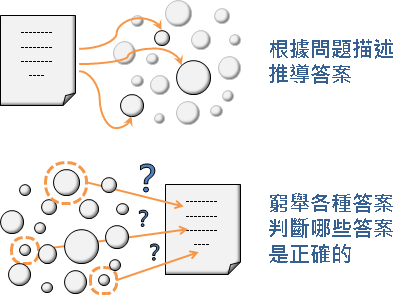
\includegraphics[scale=0.5]{images/Enumeration18}
\par\end{center}


\subsection{范例:暴力攻击( Brute Force Attack )}

破解密码最简单的方法叫做「暴力攻击」。不知道密码规律的情况下,无法直接推导正确密码,只好以试误法一一检验所有可能的密码,从中找出正确密码。

\begin{center}
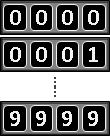
\includegraphics[scale=0.5]{images/Enumeration19}
\par\end{center}


\subsection{范例:单向函数( One-way Function )}

「单向函数」是一种特别的函数,给定输入很容易算出输出,但是给定输出却很难算出输入。

\begin{center}
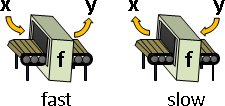
\includegraphics[scale=0.5]{images/Enumeration20}
\par\end{center}

举例来说,令一个函数的输入是两个质数,输出是两个质数的乘积。给定两个质数可以轻易的在多项式时间内算出乘积,然而给定两质数的乘积却需要指数时间才能完成质因子分解。

如果给定一个单向函数的输入,求其输出,就适合用直接法,套用函数快速算得答案;如果给定一个单向函数的输出,求其输入,就适合用试误法,尝试各种输入并套用函数快速验证答案。 


\section{Iterative Method}

\begin{flushright}
\textit{道生一,一生二,二生三,三生万物。《老子》}
\par\end{flushright}


\subsection{Iterative Method}

繁中「迭代法」、简中「递推法」。不断利用目前求得的数值,再求得新数值。

\noindent \marginpar{%
\begin{minipage}[t]{10em}%
\begin{shaded}%
UVa \protect\href{http://uva.onlinejudge.org/external/9/997.html}{997}\end{shaded}%
\end{minipage}}


\subsection{范例:字符串变整数}

\begin{center}
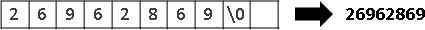
\includegraphics[scale=0.5]{images/Iterative1}
\par\end{center}

直觉的方式是递增法。个、十、百、千、万、……,每个位数分别乘上 10 的次方,通通加起来。此处按照高位数到低位数的顺序进行处理,以符合字符串的储存顺序。

\begin{center}
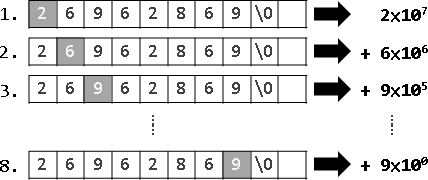
\includegraphics[scale=0.5]{images/Iterative2}
\par\end{center}

\begin{lstlisting}[language={C++},numbers=left,basicstyle={\ttfamily}]
// 计算字符串长度
int string_length(char* s)
{
    int n = 0;
    while (s[n]) n++;
    return n;
}

// 计算10的exp次方
int pow10(int exp)
{
    int n = 1;
    for (int i=0; i<exp; i++)
        n *= 10;
    return n;
}

void string_to_integer()
{
    char s[10] = "26962869";

    // 预先计算字符串长度。
    int length = string_length(s);

    // 依序处理高位数到低位数。
    int n = 0;
    for (int i=0; i<length; i++)
        n += (s[i] - '0') * pow10(length - 1 - i);

    cout << n;
}
\end{lstlisting}


更好的方式是递推法!由高位数到低位数、也就是由左到右读取字符串,每读取一个字符,就将数值乘以十、加上当前字符的对应数字。

\begin{lstlisting}[language={C++},numbers=left,basicstyle={\ttfamily}]
void string_to_integer()
{
    char s[10] = "26962869";

    int n = 0;
    for (int i=0; s[i]; i++)
        n = n * 10 + s[i] - '0';

    cout << n;
}
\end{lstlisting}


同一个问题,有着不同的解法。有着程序代码很长、执行速度很慢的方法,也有着程序代码很短,执行速度很快的方法。一支程序的好坏,除了取决于正确性和可读性之外,同时也取决于计算方法。

\noindent \marginpar{%
\begin{minipage}[t]{10em}%
\begin{shaded}%
UVa \protect\href{http://uva.onlinejudge.org/external/7/759.html}{759}\end{shaded}%
\end{minipage}}


\subsection{范例:秦九韶算法( Horner's Rule )}

多项式函数,代入数值。一乘一加,不断更迭,求得函数值。完全不需要次方运算。

\begin{center}
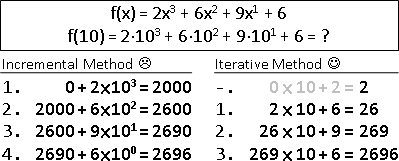
\includegraphics[scale=0.5]{images/Iterative4}
\par\end{center}


\subsection{范例: 3n+1 猜想( Collatz Conjecture )}

猜想的内容是这样的:有一个整数,如果是偶数,就除以 2 ;如果是奇数,就乘以 3 再加 1 。一个整数不断这样操作下去,最后一定会变成
1 。这个操作的过程就是一种递推。

\begin{center}
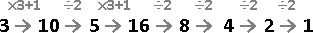
\includegraphics[scale=0.5]{images/Iterative5}
\par\end{center}

至今尚未有人能证明其正确性。有趣的是,目前也尚未检查出任何反例。

\noindent \marginpar{%
\begin{minipage}[t]{10em}%
\begin{shaded}%
UVa \protect\href{http://uva.onlinejudge.org/external/1/100.html}{100}
\protect\href{http://uva.onlinejudge.org/external/3/371.html}{371}
\protect\href{http://uva.onlinejudge.org/external/6/694.html}{694}\end{shaded}%
\end{minipage}}


\subsection{范例:除法}

不断乘以十、除以除数,就是一种递推。

\begin{center}
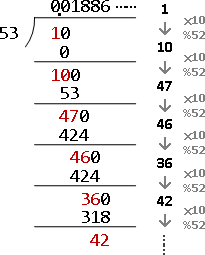
\includegraphics[scale=0.5]{images/Iterative6}
\par\end{center}


\subsection{范例:牛顿法( Newton's Method )}

一个经典的递推法范例,微积分课程一定有教过。牛顿法用来求连续函数的其中一个根。一开始先随便设定一点,不断利用斜率求出下一点。
\[
X_{n+1}=X_{n}-\frac{f(X_{n})}{f'(X_{n})}
\]


\begin{center}
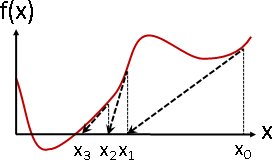
\includegraphics[scale=0.5]{images/Iterative7}
\par\end{center}


\subsection{范例:十分逼近法}

数线分割成十等份区间,从中找出正确区间,把对应的小数字数添到答案末端,然后不断十等分下去。

\begin{center}
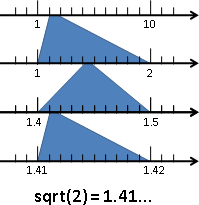
\includegraphics[scale=0.5]{images/Iterative8}
\par\end{center}


\subsection{范例:书塔( Book Stacking Problem )}

将书本一本一本迭起来,成为一座斜塔,越斜越好。

\begin{center}
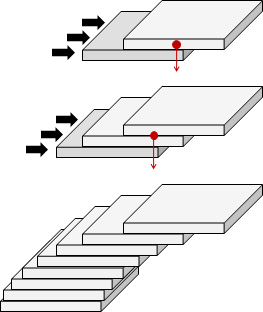
\includegraphics[scale=0.5]{images/Iterative9}
\par\end{center}

对于任何一本书来说,其上方所有书本的整体重心,必须落在这本书上,这本书才能平稳地支撑住上方所有书本。

将书本插入到书塔底部,让书塔的重心落在书本边缘,就可以让书塔最斜。插入书本到书塔底部之后,就更新书塔的重心位置,以便稍后插入下一本书本。

不断插入书本到书塔底部、更新书塔重心,运用先前的书塔求得新的书塔──这段过程就是一种递推。 


\subsection{范例:生命游戏( The Game of Life )( Cellular Automata )}

一个二维的方格平面,每个格子都有一个细胞,可能是活的,可能是死的。细胞的生命状况,随时间变动,变动规则如下:

\noindent %
\shadowbox{\begin{minipage}[t]{1\columnwidth}%
复活:一个死的细胞,若是它的八个邻居,有三个细胞是活的,则在下一刻复活。

存活:一个活的细胞,若是它的八个邻居,有两个或三个细胞是活的,则在下一刻存活。

死于孤单:一个活的细胞,若是它的八个邻居,只有零个或一个细胞是活的,则在下一刻死亡。

死于拥挤:一个活的细胞,若是它的八个邻居,有四个以上的细胞是活的,则在下一刻死亡。 %
\end{minipage}}

\begin{center}
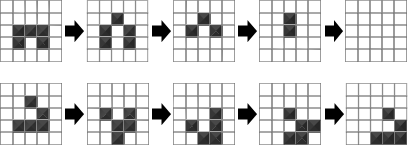
\includegraphics[scale=0.5]{images/Iterative10}
\par\end{center}

实作时,我们可以弄两张地图,第一张地图储存现在这个时刻的状态,第二张地图储存下一个时刻的状态。两张地图交替使用,以节省内存空间。

细胞的变动规则,包装成一个函数,让程序代码易读。 

\begin{lstlisting}[language={C++},numbers=left,basicstyle={\ttfamily}]
void go(int x, int y, bool map1[100][100], bool map2[100][100])
{
    int n = 八个邻居中,还活着的细胞数目;

    if (!map1[x][y])
        if (n == 3)                 // 复活
            map2[x][y] = true;
        else                        // 仍旧死亡
            map2[x][y] = map1[x][y];
    else
        if (n == 2 || n == 3)       // 存活
            map2[x][y] = true;
        else if (n == 0 || n == 1)  // 死于孤单
            map2[x][y] = false;
        else if (n >= 4)            // 死于拥挤
            map2[x][y] = false;
}

void cellular_automata()
{
    bool map[2][100][100];

    map[0][50][50] = true;  // 自行设定一些活的细胞
    map[0][50][51] = true;
    map[0][51][50] = true;

    for (int t=0; t<100; ++t)
        for (int x=0; x<100; ++x)
            for (int y=0; y<100; ++y)
                go(x, y, map[t%2], map[(t+1)%2]);
}
\end{lstlisting}


\noindent \marginpar{%
\begin{minipage}[t]{10em}%
\begin{shaded}%
UVa \protect\href{http://uva.onlinejudge.org/external/4/447.html}{447}
\protect\href{http://uva.onlinejudge.org/external/4/457.html}{457}
\protect\href{http://uva.onlinejudge.org/external/104/10443.html}{10443}
\protect\href{http://uva.onlinejudge.org/external/105/10507.html}{10507}\end{shaded}%
\end{minipage}}


\subsection{范例:兰顿的蚂蚁( Langton's Ant )}

跟生命游戏相似,不过这个游戏更神奇。

\noindent %
\shadowbox{\begin{minipage}[t]{1\columnwidth}%
一、格子有黑与白两种颜色。 

二、蚂蚁走入白格则右转,走入黑格则左转。

三、蚂蚁离开格子时,格子颜色颠倒。 %
\end{minipage}}

惊人的是,乍看完全没有规律的路线,却在 10647 步之后开始循环。原因至今不明。

\noindent \marginpar{%
\begin{minipage}[t]{10em}%
\begin{shaded}%
UVa \protect\href{http://uva.onlinejudge.org/external/116/11664.html}{11664}\end{shaded}%
\end{minipage}}


\subsection{范例:以试除法建立质数表}

从表面上来看是两层的枚举法:第一层先枚举正整数,一一试验是否为质数;第二层再枚举所有已知质数,一一试除。

但是从另一个角度来看,利用目前求得的质数,再求出更多质数,其实就是递推法。 


\subsection{范例:数学归纳法( Mathematical Induction )}

数学归纳法的第二步骤,就是证明可不可以递推!第二步骤的证明过程中一定会用到递推!

\noindent %
\shadowbox{\begin{minipage}[t]{1\columnwidth}%
1. 先证明 $n=1$ 成立。(有时候不见得要从1开始。)

2. 假设 $n=k$ 成立,证明 $n=k+1$ 也会成立。\\


当 1. 2. 得证,就表示 $n=1\cdots\infty$ 全部都成立。 %
\end{minipage}}


\section{Recursive Method}

\begin{flushright}
\textit{易有太极,是生两仪。两仪生四象,四象生八卦。《易传》}
\par\end{flushright}


\subsection{Recursive Method}

繁中「递归法」、简中「递归法」。重复运用相同手法,缩减问题范围,直到厘清细节。

\noindent \marginpar{%
\begin{minipage}[t]{10em}%
\begin{shaded}%
UVa \protect\href{http://uva.onlinejudge.org/external/109/10994.html}{10994}
\protect\href{http://uva.onlinejudge.org/external/102/10212.html}{10212}
\protect\href{http://uva.onlinejudge.org/external/104/10471.html}{10471}
\protect\href{http://uva.onlinejudge.org/external/109/10922.html}{10922}\end{shaded}%
\end{minipage}}


\subsection{范例:碎形( Fractal )}

利用相同手法绘图,绘图范围越来越精细。

图中的碎形称作 Sierpinski triangle 。凡是尖端朝上的正三角形,就在当中放置一个尖端朝下的正三角形;放置之后,图形就变得更细腻,范围就变得更小了。

\begin{center}
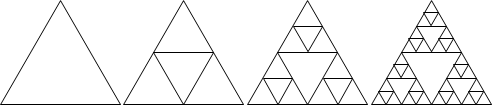
\includegraphics[scale=0.5]{images/Recursive1}
\par\end{center}

图中的碎形称作 Kosh snowflake 。一条边三等分,去除中段,朝外补上两段,形成尖角。

\begin{center}
\includegraphics[scale=0.5]{images/Recursive2}
\par\end{center}

图中的碎形称作 Pythagorean tree 。不断绘制正方形、直角三角形,看起来像是一棵茂密的树。

\begin{center}
\includegraphics[scale=0.3]{images/618px-Pythagoras_tree_1_1_13_Summer\lyxdot svg}
\par\end{center}

\noindent \marginpar{%
\begin{minipage}[t]{10em}%
\begin{shaded}%
UVa \protect\href{http://uva.onlinejudge.org/external/1/177.html}{177}
\protect\href{http://uva.onlinejudge.org/external/106/10609.html}{10609}\end{shaded}%
\end{minipage}}


\subsection{范例:质因子分解( Integer Factorization )}

不断抽取出质因子,使数值不断变小,直到成为质因子。

\begin{center}
\includegraphics[scale=0.5]{images/Recursive3}
\par\end{center}


\subsection{范例: L 形磁砖}

有一个边长为 2 的 3 次方的正方形,右上角缺了一角边长为 1 的正方形。现在要以 L 形磁砖贴满这个缺了一角的正方形,该如何贴呢?

\begin{center}
\includegraphics[scale=0.5]{images/Recursive4}
\par\end{center}

巧妙地将一块 L 形磁砖放在中央的位置,就顺利的把正方形切成四个比较小的、亦缺了一角的正方形。接下来只要递归处理四个小正方形,就解决问题了。

这个问题也可以改成缺口在任意一处,各位可以想想看怎么解。 

\noindent \marginpar{%
\begin{minipage}[t]{10em}%
\begin{shaded}%
UVa \protect\href{http://uva.onlinejudge.org/external/102/10230.html}{10230}\end{shaded}%
\end{minipage}}


\subsection{范例:辗转相除法( Euclid's Algorithm )}

两个数字轮流相除、求余数,最后就得到最大公因子( greatest common divisor, gcd )。相信大家小时候都有学过。

\begin{center}
\includegraphics[scale=0.5]{images/Recursive5}
\par\end{center}

我们可以把最大公因子想象成砖块、把两个数字都看成是最大公因子的倍数。

两数相减所得的差值,一定是最大公因子的倍数。更进一步来说,两数相除所得的余数,一定是最大公因子的倍数。辗转相除法的过程当中,两数自始至终都是最大公因子的倍数。

运用这个性质,我们把两数相除、求余数,使得原始数字不断缩小,直到得到最大公因子。真是非常巧妙的递归法! 

\begin{lstlisting}[language={C++},numbers=left,basicstyle={\ttfamily}]
// 运用程序语言的循环语法。
int gcd(int a, int b)
{
    // 令 a 比 b 大,比较容易思考。
    while (b != 0)
    {
        int t = a % b;
        a = b;
        b = t;
    }
    return a;
}
\end{lstlisting}


\noindent \rule[0.5ex]{0.7\columnwidth}{1pt}

\begin{lstlisting}[language={C++},numbers=left,basicstyle={\ttfamily}]
// 运用程序语言的递归语法。
int gcd(int a, int b)
{
    // 令 a 比 b 大,比较容易思考。
    if (b == 0)
        return a;
    else
        return gcd(b, a % b);
}
\end{lstlisting}


注意到,递推法、递归法,不等于程序语言中的循环、递归。递推法、递归法是分析问题的方法,用来得到计算过程、用来得到算法。至于编写程序时,我们可以自由地采用循环或者递归。


\subsection{递推法、递归法,一体两面,同时存在。}

递推法与递归法恰好颠倒:递推法是针对已知,逐步累积,直至周全;递归法是针对未知,反复拆解,直至精确。

递推法是由小到大,递归法是由大到小。 

\begin{center}
\includegraphics[scale=0.5]{images/Recursive6}
\par\end{center}


\subsection{范例:秦九韶算法( Horner's Rule )}

递推法是不断配 x ,扩增已知;递归法是不断提 x ,减少未知。

\noindent %
\shadowbox{\begin{minipage}[t]{1\columnwidth}%
$ax^{2}+bx+c$\\


Iterative Method:

$\{a\}*x^{2}+b*x^{1}+c$

$\{a,*x\}*x^{1}+b*x^{1}+c$

$\{a,*x,+b\}*x^{1}+c$

$\{a,*x,+b,*x\}+c$

$\{a,*x,+b,*x,+c\}$\\


Recursive Method:

$\{a*x^{2}+b*x^{1}+c\}$

$\{a*x^{2}+b*x^{1}\},+c$

$\{a*x^{1}+b\},*x,+c$

$\{a*x^{1}\},+b,*x,+c$

$\{a\},*x,+b,*x,+c$%
\end{minipage}}

\noindent 虽然递推法与递归法的推理方向是相反的,但是递推法与递归法的计算方向是一样的,两者都是由小范围算到大范围。

\noindent %
\shadowbox{\begin{minipage}[t]{1\columnwidth}%
Iterative Method:

$a,*x,+b,*x,+c$\\


Recursive Method:

$a,*x,+b,*x,+c$%
\end{minipage}}

\noindent \marginpar{%
\begin{minipage}[t]{10em}%
\begin{shaded}%
UVa \protect\href{http://uva.onlinejudge.org/external/4/498.html}{498}
\protect\href{http://uva.onlinejudge.org/external/102/10268.html}{10268}\end{shaded}%
\end{minipage}}


\subsection{范例:爬楼梯}

眼前有五阶楼梯,一次只能踏一阶或踏两阶,那么爬到五阶总共有哪几种踏法?例如 (1,1,1,1,1) 是其中一种踏法, (1,2,2)
是另一种踏法。

\begin{center}
\includegraphics[scale=0.5]{images/Recursive7}
\par\end{center}

这个问题可以用递推法,也可以用递归法。

首先采用递推法。试着只爬少少的几阶楼梯,观察一下踏法。

爬到一阶的踏法:很明显的只有一种, (1) 。

爬到两阶的踏法:有两种, (1,1) 和 (2) 。

爬到三阶的踏法:因为一次只能踏一阶或踏两阶,所以只可能从第一阶或从第二阶踏上第三阶。只要综合 ( 爬到一阶的踏法 ,2) 与 ( 爬到两阶的踏法
,1) ,就是爬到三阶的踏法。

爬到四阶的踏法:同理,综合 ( 爬到两阶的踏法 ,2) 与 ( 爬到三阶的踏法 ,1) 即得。

递推下去,就可求出爬到五阶的踏法。 

\noindent %
\begin{tabular}{cl}
\multicolumn{2}{c}{Forward Iterative Method:}\tabularnewline
爬到一阶 & (1)\tabularnewline
爬到两阶 & (1,1) (2) \tabularnewline
爬到三阶 & 即是(爬到一阶,2)与(爬到二阶,1)\tabularnewline
 & (1,2)\tabularnewline
 & (1,1,1) (2,1)\tabularnewline
爬到四阶 & 即是(爬到二阶,2)与(爬到三阶,1)\tabularnewline
 & (1,1,2) (2,2)\tabularnewline
 & (1,2,1) (1,1,1,1) (2,1,1)\tabularnewline
爬到五阶 & 即是(爬到三阶,2)与(爬到四阶,1)\tabularnewline
 & (1,2,2) (1,1,1,2) (2,1,2)\tabularnewline
 & (1,1,2,1) (2,2,1) (1,2,1,1) (1,1,1,1,1) (2,1,1,1)\tabularnewline
\end{tabular}

前面是采用上楼梯的顺序进行递推,由第一阶递推到第五阶。也可以采用下楼梯的顺序进行递推,由第五阶递推到第一阶。

\noindent %
\begin{tabular}{cl}
\multicolumn{2}{c}{Backward Iterative Method:}\tabularnewline
降到四阶 & (1)\tabularnewline
降到三阶 & (1,1) (2) \tabularnewline
降到二阶 & 即是(2,降到四阶)与(1,降到三阶)\tabularnewline
 & (1,2)\tabularnewline
 & (1,1,1) (2,1)\tabularnewline
降到一阶 & 即是(2,降到三阶)与(1,降到二阶)\tabularnewline
 & (1,1,2) (2,2)\tabularnewline
 & (1,2,1) (1,1,1,1) (2,1,1)\tabularnewline
降到平面 & 即是(2,降到二阶)与(1,降到一阶)\tabularnewline
 & (1,2,2) (1,1,1,2) (2,1,2)\tabularnewline
 & (1,1,2,1) (2,2,1) (1,2,1,1) (1,1,1,1,1) (2,1,1,1)\tabularnewline
\end{tabular}

有一些问题,比如爬楼梯问题,双向都可以递推。数值由小到大的方向称为「正向」或「顺向」( forward ),数值由大到小的方向称为「反向」或「逆向」(
backward )。

接着采用递归法。由踏出的最后一步开始分析。

要「爬到五阶」,最后一步一定是踏上第五阶。要踏上第五阶,只可能从第四阶和第三阶踏过来,也就是综合 ( 爬到四阶的踏法 ,1) 与 (
爬到三阶的踏法 ,2) 。

但是我们尚不知如何「爬到四阶」和「爬到三阶」,所以只好再分别研究「爬到四阶」与「爬到三阶」。不断追究到「爬到一阶」与「爬到两阶」的时候,就能确认答案了! 

\noindent %
\shadowbox{\begin{minipage}[t]{1\columnwidth}%
Forward(?) Recursive Method:

爬到五阶 即是(爬到四阶,1)与(爬到三阶,2)

爬到四阶 即是(爬到三阶,1)与(爬到二阶,2)

爬到三阶 即是(爬到二阶,1)与(爬到一阶,2)

爬到两阶 (2) (1,1)

爬到一阶 (1) %
\end{minipage}}

当然也可以双向递归。就不赘述了。


\subsection{范例:格雷码( Gray Code )}

\noindent %
\shadowbox{\begin{minipage}[t]{1\columnwidth}%
Iterative Method:

GrayCode(n-1)的每个数字,最高位数加一个0。

GrayCode(n-1)的每个数字,高位数与低位数整个颠倒,然后在最高位数加一个1。

两者衔接起来就是GrayCode(n)。\\


Recursive Method:

GrayCode(n)的每个数字,分成两类。

第一类最高位数是0,把最高位数拿掉后,即形成GrayCode(n-1)。

第二类最高位数是1,把最高位数拿掉后,即形成GrayCode(n-1)。 %
\end{minipage}}

也可以用最低位数为主,进行递推、递归,生成顺序不同的 Gray Code 。 Gray Code 具有循环的特性,有多种递推、递归方式,不分正向与逆向。


\section{Divide and Conquer}

\begin{flushright}
\textit{凡治众如治寡,分数是也。斗众如斗寡,形名是也。《孙子》}
\par\end{flushright}


\subsection{Divide and Conquer}

「分治法」,分割问题、各个击破。将一个大问题,分割成许多小问题。如果小问题还是很难,就继续分割成更小的问题,直到问题变得容易解决。

分割出来的小问题,称作「子问题 subproblem 」。解决一个问题,等价于解决所有子问题。 

用树形图表达原问题与子问题的关系,最好不过! 

\begin{center}
\includegraphics[scale=0.5]{images/DivideAndConquer1}
\par\end{center}

分治法着重分割问题的方式──要怎么分割问题,使得子问题简单又好算?各位读者可以藉由本文的范例,体会分割问题的方式。


\subsection{范例:分解动作}

想要学习「从中场带球上篮」,我们可以将此动作分割为「跑步运球」、「跑步收球」、「单手将球放入篮框」等动作,分别学习。每一项动作都熟练之后,组合起来便是带球上篮了。

如果觉得「跑步运球」还是太难,可以更细分成「原地运球」、「走动运球」、「运球时护球」等动作,克服了之后便能够顺利解决「跑步运球」的问题了。 

\begin{center}
\includegraphics[scale=0.5]{images/DivideAndConquer2}
\par\end{center}


\subsection{范例:方格法求面积}

左边为原问题,右边放大并细分的图是其中一个子问题。

\begin{center}
\includegraphics[scale=0.5]{images/DivideAndConquer3}
\par\end{center}


\subsection{范例:分类数数}

左边最大的框框是原问题,将原问题的数字进行分类后再统计,分类后的每一个框框都是一个子问题。

\begin{center}
\includegraphics[scale=0.5]{images/DivideAndConquer4}
\par\end{center}

\noindent \marginpar{%
\begin{minipage}[t]{10em}%
\begin{shaded}%
UVa \protect\href{http://uva.onlinejudge.org/external/110/11038.html}{11038}\end{shaded}%
\end{minipage}}


\subsection{Recursive Method}

在分治法当中,亦得递归地分割问题,其实就是递归法。

\begin{center}
\includegraphics[scale=0.5]{images/DivideAndConquer5}
\par\end{center}

程序代码细分为三个阶段: Divide 、 Conquer 、 Combine 。 Divide 阶段是把原问题分割成小问题, Conquer
阶段是解决小问题, Combine 阶段是运用小问题的解答,整理出原问题的解答。

\begin{center}
\includegraphics[scale=0.5]{images/DivideAndConquer6}
\par\end{center}

\begin{lstlisting}[language={C++},numbers=left,basicstyle={\ttfamily}]
divide_and_conquer(原问题)
{
    /* Divide */
    先将原问题分割成许多小问题;

    /* Conquer */
    递归调用函数,求得子问题的解;
    解答1 = divide_and_conquer(子问题1);
    解答2 = divide_and_conquer(子问题2);
    ......

    /* Combine */
    用小问题的解答,算出原问题的解答;
    原问题解答 = 解答1 + 解答2 + ......;

    return 原问题解答;
}
\end{lstlisting}


\noindent \marginpar{%
\begin{minipage}[t]{10em}%
\begin{shaded}%
UVa \protect\href{http://uva.onlinejudge.org/external/6/620.html}{620}
\protect\href{http://uva.onlinejudge.org/external/101/10101.html}{10101}
\protect\href{http://uva.onlinejudge.org/external/101/10144.html}{10144}
\protect\href{http://uva.onlinejudge.org/external/109/10998.html}{10998}\end{shaded}%
\end{minipage}}


\subsection{范例:归并排序法( Merge Sort )}

\begin{center}
\includegraphics[scale=0.5]{images/DivideAndConquer7}
\par\end{center}

Divide 阶段:数据分割成两堆。 

Conquer 阶段:两堆资料各自从事 Merge Sort 。 

Combine 阶段:两堆已排序过的数据,合并成一堆。 


\subsection{范例:快速排序法( Quicksort )}

\begin{center}
\includegraphics[scale=0.5]{images/DivideAndConquer8}
\par\end{center}

Divide 阶段:选择一个数值当作基准,把数据分割成左右两堆,使得左堆数值小于基准,右堆数值大于基准,基准数值置于左右两堆中间。

Conquer 阶段:左右两堆资料各自从事 Quicksort 。

Combine 阶段:不做任何事。 


\subsection{范例:不重复组合( Combination )}

从 N 个人抓 M 个人出来组团,有哪些组合方式呢?

\begin{center}
\includegraphics[scale=0.5]{images/DivideAndConquer9}
\par\end{center}

N 个人当中的其中一个人,叫做甲君好了,我们将原问题分割成两种情形:甲君在团中、甲君不在团中。

\noindent %
\shadowbox{\begin{minipage}[t]{1\columnwidth}%
甲君在团中,演变成剩下N-1个人要再抓M-1个人出来组团。

甲君不在团中,演变成剩下N-1个人仍要抓M个人出来组团。 %
\end{minipage}}

综合这两个子问题的组合方式,就得到答案。


\subsection{范例:汉诺塔( Tower of Hanoi )}

三根柱子、一迭盘子,盘子大小皆不同(盘子中间还得打个洞,这样盘子才能穿在柱子上)。所有盘子都迭在第一根柱子,大的在下面,小的在上面。现在要将整迭盘子移到第三根柱子,并且保持原来的大小顺序。每次只能搬动一个盘子到别根柱子,而且大的盘子一定要保持在小的盘子下面。

\begin{center}
\includegraphics[scale=0.5]{images/DivideAndConquer10}
\par\end{center}

想要移动最大的盘子到第三根柱子,必须先挪开上方整迭盘子到第二根柱子。移动上方整迭盘子,正好与原问题相同、而少了一个盘子,可以视作子问题。

\begin{center}
\includegraphics[scale=0.5]{images/DivideAndConquer11}
\par\end{center}

尝试以此子问题解决原问题,解题过程因而简化成三个步骤:一、上方整迭盘子移到第二根柱子;二、最大的盘子移到第三根柱子;三、方才的整迭盘子移到第三根柱子。

\begin{center}
\includegraphics[scale=0.5]{images/DivideAndConquer12}
\par\end{center}

\begin{lstlisting}[language={C++},numbers=left,basicstyle={\ttfamily}]
int p[5];   // 盘子所在的柱子。第i小的盘子放在第p[i]根柱子。

void move(int n, int t) // 将前n小的盘子移到第t根柱子
{
    if (n == 0) return;
    move(n-1, 6-p[n]-t);
    cout << "从" << p[n] << "移到" << t;
    p[n] = t;
    move(n-1, t);
}

void tower_of_hanoi()
{
    // 五个盘子,都迭在第一根柱子。
    for (int i=1; i<=5; ++i) p[i] = 1;
    // 五个盘子,从第一根柱子移到第三根柱子。
    move(5, 3);
}
\end{lstlisting}


\noindent \marginpar{%
\begin{minipage}[t]{10em}%
\begin{shaded}%
UVa \protect\href{http://uva.onlinejudge.org/external/100/10017.html}{10017}\end{shaded}%
\end{minipage}}

\noindent \clearpage{}
\end{document}
